\documentclass[11pt]{article}
\usepackage[margin=1in]{geometry}
\usepackage{amsmath,amssymb,amsthm}
\usepackage{booktabs}
\usepackage{graphicx}
\usepackage[hidelinks]{hyperref}
\usepackage{array}
\usepackage{enumitem}
\graphicspath{{../figures/}{figures/}{./}}

\newtheorem{theorem}{Theorem}
\newtheorem{proposition}{Proposition}
\newtheorem{lemma}{Lemma}
\theoremstyle{definition}
\newtheorem{definition}{Definition}
\newtheorem{assumption}{Assumption}
\theoremstyle{remark}
\newtheorem{remark}{Remark}

\renewcommand{\Pr}{\operatorname{Pr}}
\newcommand{\E}{\operatorname{E}}
\newcommand{\Var}{\operatorname{Var}}
\newcommand{\Bin}{\operatorname{Binomial}}
\newcommand{\Ber}{\operatorname{Bernoulli}}
\newcommand{\Betad}{\operatorname{Beta}}
\newcommand{\Bfun}{\mathrm{B}}
\newcommand{\ind}[1]{\mathbf{1}\{#1\}}
\newcommand{\data}{\text{data}}
\newcommand{\rulename}[1]{\ {[\emph{#1}]}}

% --- generated files (the scripts write these; the report still compiles without them)
\IfFileExists{sim_macros.tex}{% Generated by src/simulation.py -- do not edit by hand
\newcommand{\simxA}{92}\newcommand{\simxB}{121}\newcommand{\simn}{1000}
\newcommand{\simM}{100{,}000}
}{%
  \newcommand{\simxA}{92}\newcommand{\simxB}{121}\newcommand{\simn}{1000}\newcommand{\simM}{100{,}000}}
\IfFileExists{data_macros.tex}{% Generated by src/load_data.py -- do not edit by hand
\newcommand{\dataRows}{90{,}189}
\newcommand{\dataCols}{5}
\newcommand{\dataMissing}{0}
}{%
  \newcommand{\dataRows}{\emph{(run \texttt{src/load\_data.py})}}
  \newcommand{\dataCols}{5}
  \newcommand{\dataMissing}{\emph{(run \texttt{src/load\_data.py})}}}

% --- Iteration 3: numbers written by src/small_example.py, check_simulation.py, run_real.py, check_assumptions.py
% Generated by src/small_example.py -- do not edit by hand
\newcommand{\smThetaExact}{\tfrac{521}{646}}
\newcommand{\smThetaExactDec}{0.806502}
\newcommand{\smThetaSwap}{\tfrac{125}{646}}
\newcommand{\smThetaMC}{0.80802}
\newcommand{\smSE}{0.00125}
\newcommand{\smNSE}{1.22}
\newcommand{\smMCerr}{0.00152}
\newcommand{\smThetaGrid}{0.8065015480}
\newcommand{\smGridErr}{2.6\times10^{-12}}
\newcommand{\smGridEight}{0.672664}
\newcommand{\smGridEightErr}{1.3\times10^{-1}}
\newcommand{\smGridForty}{0.80648863}
\newcommand{\smGridFortyErr}{1.3\times10^{-5}}
\newcommand{\smGridTwoHundred}{0.8065015219}
\newcommand{\smGridTwoHundredErr}{2.6\times10^{-8}}
\newcommand{\smZ}{0.9129}
\newcommand{\smP}{0.3613}
\newcommand{\smPone}{0.1807}
\newcommand{\smOneMinusTheta}{0.1935}
\newcommand{\smConjErr}{8.1\times10^{-12}}
\newcommand{\smIntfA}{0.999999999997}
\newcommand{\smDrawsA}{0.3710,\ 0.2033,\ 0.2922,\ 0.3037,\ 0.3673}
\newcommand{\smDrawsB}{0.3857,\ 0.4853,\ 0.5514,\ 0.4792,\ 0.3634}
\newcommand{\smInd}{1,\ 1,\ 1,\ 1,\ 0}
\newcommand{\smRunTen}{0.900}
\newcommand{\smRunThousand}{0.802}
\newcommand{\smSampleMeanA}{0.3328}
\newcommand{\smSampleMeanB}{0.5003}

% Generated by src/check_simulation.py -- do not edit by hand
\newcommand{\simThetaMC}{0.98288}
\newcommand{\simSE}{0.00041}
\newcommand{\simThetaGrid}{0.98213167}
\newcommand{\simThetaLib}{0.98213167}
\newcommand{\simGridErr}{4.0\times10^{-12}}
\newcommand{\simNSE}{1.82}
\newcommand{\simZ}{2.1021}
\newcommand{\simP}{0.0355}
\newcommand{\simMomErr}{0}
\newcommand{\simPdfErr}{1.5\times10^{-13}}
\newcommand{\simZErr}{0}
\newcommand{\simPErr}{1.4\times10^{-17}}
\newcommand{\simMuA}{0.09281}
\newcommand{\simMuB}{0.12176}
\newcommand{\simSdA}{0.00916}
\newcommand{\simSdB}{0.01033}
\newcommand{\simSlopeA}{-0.502}
\newcommand{\simSlopeB}{-0.503}
\newcommand{\simTruthErr}{0.0074}
\newcommand{\simTruthSE}{0.78}
\newcommand{\simNullRej}{0.040}
\newcommand{\simNullZsd}{0.966}
\newcommand{\simNullZmean}{0.048}
\newcommand{\strBoth}{100}
\newcommand{\strRows}{2000}
\newcommand{\strUnique}{1900}
\newcommand{\strDup}{100}
\newcommand{\strXA}{97/1000}
\newcommand{\strXB}{140/1000}
\newcommand{\strXAc}{79/900}
\newcommand{\strXBc}{122/900}
\newcommand{\strCleanNullRej}{0.0515}
\newcommand{\strNullRej}{0.0393}
\newcommand{\strNullRejTheory}{0.0388}
\newcommand{\strNullSdZ}{0.950}
\newcommand{\strCleanNullSdZ}{1.004}
\newcommand{\strNullCorr}{0.101}
\newcommand{\strCleanCorr}{+0.001}
\newcommand{\strAltDiff}{0.0182}
\newcommand{\strCleanAltDiff}{0.0202}
\newcommand{\strAltPower}{0.243}
\newcommand{\strCleanAltPower}{0.303}
\newcommand{\strSdAssumed}{0.0134}
\newcommand{\strSdTrue}{0.0127}
\newcommand{\strNullSd}{0.0127}

% Generated by src/run_real.py -- do not edit by hand
\newcommand{\realRaw}{90{,}189}
\newcommand{\realMissing}{0}
\newcommand{\realDup}{0}
\newcommand{\realBoth}{0}
\newcommand{\realRemoved}{0}
\newcommand{\realClean}{90{,}189}
\newcommand{\realUnique}{90{,}189}
\newcommand{\realNA}{44{,}700}
\newcommand{\realNB}{45{,}489}
\newcommand{\realRatio}{0.9827}
\newcommand{\realFewer}{1.7}
\newcommand{\realShareA}{0.4956}
\newcommand{\realOneXA}{20{,}034}
\newcommand{\realOneXB}{20{,}119}
\newcommand{\realOneRateA}{0.4482}
\newcommand{\realOneRateB}{0.4423}
\newcommand{\realOneTheta}{0.0372}
\newcommand{\realOneThetaA}{0.9628}
\newcommand{\realOneMC}{0.03668}
\newcommand{\realOneSE}{0.00059}
\newcommand{\realOneNSE}{0.88}
\newcommand{\realOneZ}{-1.784}
\newcommand{\realOneP}{0.0744}
\newcommand{\realOnePhalf}{0.03720}
\newcommand{\realOneThetaFive}{0.03721}
\newcommand{\realOneSdA}{0.0024}
\newcommand{\realOneSdB}{0.0023}
\newcommand{\realOneMuA}{0.4482}
\newcommand{\realOneMuB}{0.4423}
\newcommand{\realOneDiff}{-0.0059}
\newcommand{\realOneLo}{-0.0124}
\newcommand{\realOneHi}{+0.0006}
\newcommand{\realOneGridErr}{1.1\times10^{-12}}
\newcommand{\realOneMomErr}{0}
\newcommand{\realOneZErr}{2.1\times10^{-14}}
\newcommand{\realOnePdfErr}{1.5\times10^{-11}}
\newcommand{\realOnePErr}{3.0\times10^{-15}}
\newcommand{\realOneSensHalf}{0.03720}
\newcommand{\realOneSensOne}{0.03721}
\newcommand{\realOneSensTwo}{0.03721}
\newcommand{\realOneSensRange}{3.4\times10^{-6}}
\newcommand{\realSevenXA}{8{,}502}
\newcommand{\realSevenXB}{8{,}279}
\newcommand{\realSevenRateA}{0.1902}
\newcommand{\realSevenRateB}{0.1820}
\newcommand{\realSevenTheta}{0.0008}
\newcommand{\realSevenThetaA}{0.9992}
\newcommand{\realSevenMC}{0.00068}
\newcommand{\realSevenSE}{0.00008}
\newcommand{\realSevenNSE}{1.18}
\newcommand{\realSevenZ}{-3.164}
\newcommand{\realSevenP}{0.0016}
\newcommand{\realSevenPhalf}{0.00078}
\newcommand{\realSevenThetaFive}{0.00078}
\newcommand{\realSevenSdA}{0.0019}
\newcommand{\realSevenSdB}{0.0018}
\newcommand{\realSevenMuA}{0.1902}
\newcommand{\realSevenMuB}{0.1820}
\newcommand{\realSevenDiff}{-0.0082}
\newcommand{\realSevenLo}{-0.0133}
\newcommand{\realSevenHi}{-0.0031}
\newcommand{\realSevenGridErr}{3.4\times10^{-12}}
\newcommand{\realSevenMomErr}{0}
\newcommand{\realSevenZErr}{5.9\times10^{-15}}
\newcommand{\realSevenPdfErr}{2.0\times10^{-12}}
\newcommand{\realSevenPErr}{4.9\times10^{-17}}
\newcommand{\realSevenSensHalf}{0.00078}
\newcommand{\realSevenSensOne}{0.00078}
\newcommand{\realSevenSensTwo}{0.00078}
\newcommand{\realSevenSensRange}{2.7\times10^{-7}}

% Generated by src/check_assumptions.py -- do not edit by hand
\newcommand{\asSimXA}{24.0}
\newcommand{\asSimXAp}{0.004}
\newcommand{\asSimXB}{6.4}
\newcommand{\asSimXBp}{0.703}
\newcommand{\asSimDup}{0}
\newcommand{\asSimRA}{-0.0184}
\newcommand{\asSimRAz}{-0.58}
\newcommand{\asSimRB}{-0.0191}
\newcommand{\asSimRBz}{-0.61}
\newcommand{\asSimBoth}{0}
\newcommand{\asSimSplitZ}{-0.31}
\newcommand{\asSimSplitP}{0.7542}
\newcommand{\asSimNA}{993}
\newcommand{\asSimNB}{1{,}007}
\newcommand{\asSimTheta}{0.99679}
\newcommand{\asSimPriorRange}{1.7\times10^{-4}}
\newcommand{\asSimW}{0.99799}
\newcommand{\asSimSmallest}{111}
\newcommand{\asSimMcSd}{0.00039}
\newcommand{\asSimMcSe}{0.00040}
\newcommand{\asSimMcRatio}{0.97}
\newcommand{\asSimAlarm}{0.062}
\newcommand{\asOneXA}{5.0}
\newcommand{\asOneXAp}{0.838}
\newcommand{\asOneXB}{7.0}
\newcommand{\asOneXBp}{0.637}
\newcommand{\asOneDup}{0}
\newcommand{\asOneRA}{+0.0025}
\newcommand{\asOneRAz}{+0.52}
\newcommand{\asOneRB}{-0.0067}
\newcommand{\asOneRBz}{-1.43}
\newcommand{\asOneBoth}{0}
\newcommand{\asOneSplitZ}{-2.63}
\newcommand{\asOneSplitP}{0.0086}
\newcommand{\asOneNA}{44{,}700}
\newcommand{\asOneNB}{45{,}489}
\newcommand{\asOneTheta}{0.03721}
\newcommand{\asOnePriorRange}{3.4\times10^{-6}}
\newcommand{\asOneW}{0.99996}
\newcommand{\asOneSmallest}{19{,}901}
\newcommand{\asOneMcSd}{0.00138}
\newcommand{\asOneMcSe}{0.00134}
\newcommand{\asOneMcRatio}{1.03}
\newcommand{\asSevenXA}{5.4}
\newcommand{\asSevenXAp}{0.799}
\newcommand{\asSevenXB}{5.6}
\newcommand{\asSevenXBp}{0.777}
\newcommand{\asSevenDup}{0}
\newcommand{\asSevenRA}{+0.0009}
\newcommand{\asSevenRAz}{+0.18}
\newcommand{\asSevenRB}{+0.0017}
\newcommand{\asSevenRBz}{+0.35}
\newcommand{\asSevenBoth}{0}
\newcommand{\asSevenSplitZ}{-2.63}
\newcommand{\asSevenSplitP}{0.0086}
\newcommand{\asSevenNA}{44{,}700}
\newcommand{\asSevenNB}{45{,}489}
\newcommand{\asSevenTheta}{0.00078}
\newcommand{\asSevenPriorRange}{2.7\times10^{-7}}
\newcommand{\asSevenW}{0.99996}
\newcommand{\asSevenSmallest}{8{,}317}
\newcommand{\asSevenMcSd}{0.00021}
\newcommand{\asSevenMcSe}{0.00020}
\newcommand{\asSevenMcRatio}{1.07}
\newcommand{\asMissing}{0}
\newcommand{\asMaxRounds}{49{,}854}
\newcommand{\asZeroA}{0.0433}
\newcommand{\asZeroB}{0.0452}
\newcommand{\asMedA}{17}
\newcommand{\asMedB}{16}
\newcommand{\asStrataLow}{0.013}
\newcommand{\asStrataHigh}{0.555}

% Generated by src/small_example.py -- do not edit by hand
\newcommand{\rowsSmall}{Small example & $\mu_A,\mu_B,\sigma_A^2,\sigma_B^2$ & exact fractions & $0$ & \checkmark \\
Small example & $\int_0^1\pi(p\mid x)\,dp$ & 1 (exact fractions) & 0 & \checkmark \\
Small example & $\theta$ (grid, 2000) & exact fraction & $2.6\times10^{-12}$ & \checkmark \\
Small example & $\hat\theta_M$ (Monte Carlo) & exact fraction & $0.0015$ ($1.22$ SE) & \checkmark \\
Small example & $z$ & $\sqrt{5/6}$ (exact) & $0$ & \checkmark \\}

% Generated by src/check_simulation.py -- do not edit by hand
\newcommand{\rowsSim}{Simulation ($n=1000$) & $(\mu_A,\mu_B)$ & true $(p_A,p_B)$ & $\|\cdot\|_2=0.0074$ ($0.78$ SE) & \checkmark \\
Simulation ($n=1000$) & $\theta$ (grid) & \texttt{integrate.quad} & $4.0\times10^{-12}$ & \checkmark \\
Simulation ($n=1000$) & $\hat\theta_M$ (Monte Carlo) & \texttt{integrate.quad} & $0.0007$ ($1.82$ SE) & \checkmark \\
Simulation ($n=1000$) & $\mu_A,\mu_B,\sigma^2_A,\sigma^2_B$ & \texttt{stats.beta} & max$|\cdot|=0$ & \checkmark \\
Simulation ($n=1000$) & $z^2$ & \texttt{chi2\_contingency} & $0$ & \checkmark \\
Simulation ($n=50\ldots50{,}000$) & slope of RMSE$(\mu_A)$ vs $n$ & $-\tfrac12$ (theory) & $0.002$ & \checkmark \\
Simulation (null, 1000 runs) & rejection rate of the $z$ test & $\alpha=0.05$ & $0.010$ & \checkmark \\
Simulation (stress test) & users in both groups found & 100 planted & $0$ & \checkmark \\
Simulation (stress test) & mean of $\hat p_B-\hat p_A$ & $(1-f)(p_B-p_A)=0.018$ & $0.0002$ & \checkmark \\}

% Generated by src/run_real.py -- do not edit by hand
\newcommand{\rowsReal}{Real data (1-day) & $\mu_A,\mu_B,\sigma^2_A,\sigma^2_B$ & \texttt{stats.beta} & max$|\cdot|=0$ & \checkmark \\
Real data (1-day) & $\theta$ (grid) & \texttt{integrate.quad} & $1.1\times10^{-12}$ & \checkmark \\
Real data (1-day) & $\hat\theta_M$ (Monte Carlo) & \texttt{integrate.quad} & $5.3\times10^{-4}$ ($0.88$ SE) & \checkmark \\
Real data (1-day) & $z^2$ & \texttt{chi2\_contingency} & rel.\ $2.1\times10^{-14}$ & \checkmark \\
Real data (7-day) & $\mu_A,\mu_B,\sigma^2_A,\sigma^2_B$ & \texttt{stats.beta} & max$|\cdot|=0$ & \checkmark \\
Real data (7-day) & $\theta$ (grid) & \texttt{integrate.quad} & $3.4\times10^{-12}$ & \checkmark \\
Real data (7-day) & $\hat\theta_M$ (Monte Carlo) & \texttt{integrate.quad} & $9.7\times10^{-5}$ ($1.18$ SE) & \checkmark \\
Real data (7-day) & $z^2$ & \texttt{chi2\_contingency} & rel.\ $5.9\times10^{-15}$ & \checkmark \\}

\title{DS5020 Final Project -- Final Report\\
  \large Project 7: Bayesian A/B Testing on the Cookie Cats Experiment}
\author{Amiya Sekhar (solo team; project leader)\\
  DS5020 Intro Linear Algebra \& Probability, Fall 2026}
\date{December 5, 2026}

\begin{document}
\maketitle

\begin{abstract}
Cookie Cats is a mobile game that tested moving its first gate from level 30 (version $A$) to level 40
(version $B$). Each of \realRaw{} new players was randomly given one of the two versions. We ask whether the move
changes the share of players who come back 1 day and 7 days after installing, and how sure we can be.
The number of returning players in each version is modelled as $\Bin(n,p)$ with a $\Betad(1,1)$ prior on $p$,
which gives a Beta posterior in closed form. The quantity we report, $\theta=\Pr(p_B>p_A\mid\data)$, is computed by
Monte Carlo and by numerical integration, and a two-proportion $z$ test is the frequentist comparison.
The method is derived by hand, worked on a 10-player example with exact fractions, implemented from scratch with
NumPy, and verified against a known truth in simulation and against SciPy; all 22 verification checks pass.
On the real data, moving the gate to level 40 lowers 7-day retention: $\Pr(p_A>p_B\mid\data)=\realSevenThetaA$,
the posterior mean of $p_B-p_A$ is $\realSevenDiff$ with 95\% interval $[\realSevenLo,\ \realSevenHi]$ (about 8 fewer
of every 1{,}000 players still playing after a week), and the $z$ test gives $p$-value $\realSevenP$. For 1-day
retention the evidence points the same way but is weaker ($\realOneThetaA$; $p$-value $\realOneP$). We recommend
keeping the gate at level 30, with one caveat: the two groups are less evenly split than a fair coin would give.
\end{abstract}

\section*{Ownership}
This is a one-person team, so every item below is owned by Amiya Sekhar. The ``checked'' column says how each
item was checked a second way.
\begin{center}
\resizebox{\textwidth}{!}{%
\begin{tabular}{llll}\toprule
Item & Owner & Checked & Status\\ \midrule
Introduction, results, limitations, conclusion (\S\ref{sec:intro}, \S\ref{sec:it3-real}--\S\ref{sec:conclusion}) & Amiya Sekhar & numbers from the scripts & done\\
Data and cleaning (\S\ref{sec:data}) & Amiya Sekhar & script checks & done\\
Method and algorithm (\S\ref{sec:method}) & Amiya Sekhar & self-checked & done\\
Code \texttt{src/methods.py}, \texttt{simulate.py} (\S\ref{sec:impl}) & Amiya Sekhar & library comparison & done\\
Verification: simulation, stress test, verification table (\S\ref{sec:verification}) & Amiya Sekhar & truth and library & done\\
Assumptions and their checks (\S\ref{sec:limits}) & Amiya Sekhar & simulated data first & done\\
Notation, definitions, Theorems~\ref{thm:binom}--\ref{thm:z} (Appendix~\ref{sec:appendix-math}) & Amiya Sekhar & self-checked, simulation & done\\
Hand-worked example (Appendix~\ref{sec:small}) & Amiya Sekhar & exact fractions, second-way checks & done\\
\bottomrule
\end{tabular}}
\end{center}

\tableofcontents
\clearpage

% =====================================================================
\section{Introduction}\label{sec:intro}

\textbf{The question.} Cookie Cats is a mobile game in which players meet a gate at a fixed level. The
company ran an experiment: each new player was randomly given version $A$, with the first gate at level 30, or
version $B$, with the first gate at level 40. For each player the data record whether they came back 1 day and
7 days after installing, so we ask:
\begin{quote}
Does moving the gate from level 30 to level 40 change the share of players who come back 1 day and 7 days after
installing the game, and how sure can we be?
\end{quote}
We write $p_A$ and $p_B$ for the true share of players who come back in version $A$ and version $B$. These are
unknown; the data tell us about them.

\textbf{Two ways to answer.} The \emph{Bayesian} answer is a probability about the rates themselves,
$\theta=\Pr(p_B>p_A\mid\data)$: the chance that level 40 keeps more players, given what we saw. The
\emph{frequentist} answer is the two-proportion $z$ test of $H_0:p_A=p_B$: how surprising the observed gap would be
if the two versions kept the same share of players. We compute both and explain why they agree.

\textbf{Words used in the math.} The derivations are written for a general A/B test, so they say \emph{visitor}
for a player and \emph{click} for a player coming back. One player is one yes-or-no trial.

\textbf{What this report contains.} \S\ref{sec:data} describes and checks the data. \S\ref{sec:method} states the
model and the algorithm; every derivation is in Appendix~\ref{sec:appendix-math}. \S\ref{sec:impl} describes the
from-scratch code. \S\ref{sec:verification} shows that the code is right: on a hand-worked example, on simulated
data whose truth we know, and against SciPy. \S\ref{sec:it3-real} gives the results on the real data and what they
mean, \S\ref{sec:limits} checks the assumptions and lists the limitations, and \S\ref{sec:conclusion} gives the
recommendation.

% =====================================================================
\section{Data}\label{sec:data}

\textbf{Source.} ``Mobile Games A/B Testing -- Cookie Cats'' (Kaggle), file \texttt{cookie\_cats.csv};
loaded by \texttt{src/load\_data.py} with \texttt{pandas}.

\textbf{Shape and variables.} \dataRows{} rows (players) and \dataCols{} columns:
\begin{center}
\begin{tabular}{llp{7.5cm}}\toprule
column & type & meaning\\ \midrule
\texttt{userid} & integer & anonymous player id (one row per player)\\
\texttt{version} & categorical & \texttt{gate\_30} (version $A$) or \texttt{gate\_40} (version $B$)\\
\texttt{sum\_gamerounds} & integer & rounds played during the first 14 days after install\\
\texttt{retention\_1} & boolean & came back 1 day after installing ($Y_i$ for the 1-day test)\\
\texttt{retention\_7} & boolean & came back 7 days after installing ($Y_i$ for the 7-day test)\\
\bottomrule
\end{tabular}
\end{center}
\textbf{Missing values:} \dataMissing{} missing entries in total (per-column counts are printed by the script).
The design is balanced by randomisation (about 45{,}000 players per version). \texttt{sum\_gamerounds} is very
right-skewed with a handful of extreme values; it is not used by the method but is a useful covariate for the
checks in \S\ref{sec:assumptions}.


% =====================================================================
\subsection{Connecting the data to the math}\label{sec:data-math}

The real dataset is the \emph{Cookie Cats} mobile-game experiment (Kaggle): new players were
randomly assigned to see the first ``gate'' at level 30 (version $A$, \texttt{gate\_30}) or at
level 40 (version $B$, \texttt{gate\_40}).
\begin{itemize}[nosep]
\item \textbf{One row} of the data matrix is one player, i.e.\ one Bernoulli \emph{trial}.
\item \textbf{One column} is one recorded variable: \texttt{userid}, \texttt{version},
      \texttt{sum\_gamerounds} (rounds played in the first 14 days), \texttt{retention\_1},
      \texttt{retention\_7}.
\item \textbf{One entry} such as \texttt{retention\_7} for player $i$ is the outcome
      $Y_i\in\{0,1\}$: a ``click'' is the player returning to the game 7 days (or 1 day) after installing.
\item $n_A$ = number of rows with \texttt{version = gate\_30}; $x_A$ = number of those rows with
      \texttt{retention\_7 = True}; likewise $n_B$, $x_B$ for \texttt{gate\_40}.
\end{itemize}
Everything the method needs from the data is therefore the four counts $(n_A,x_A,n_B,x_B)$,
one set for 1-day retention and one for 7-day retention.

\IfFileExists{data_summary.tex}{% Generated by src/load_data.py -- do not edit by hand
\begin{table}[ht]\centering\caption{Cookie Cats: trials $n$ and successes $x$ per version.}\label{tab:data}
\begin{tabular}{lrrrrr}\toprule version & $n$ & $x$ (1-day) & $x/n$ & $x$ (7-day) & $x/n$ \\ \midrule
gate\_30 (A) & 44{,}700 & 20{,}034 & 0.4482 & 8{,}502 & 0.1902 \\
gate\_40 (B) & 45{,}489 & 20{,}119 & 0.4423 & 8{,}279 & 0.1820 \\
\bottomrule\end{tabular}\end{table}
}{%
\begin{center}\emph{Table~\ref{tab:data} ($n$ and $x$ per version) is generated by \texttt{src/load\_data.py}
once \texttt{data/cookie\_cats.csv} is in place.}\end{center}}

\begin{figure}[ht]\centering
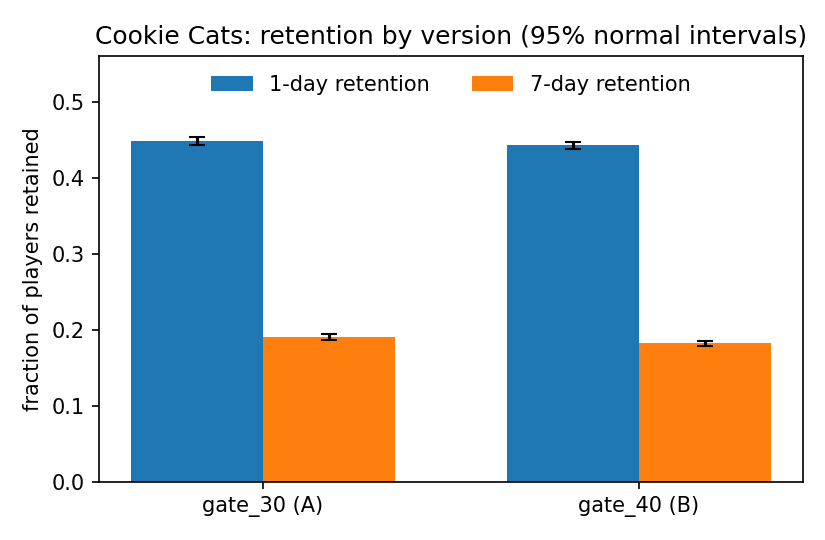
\includegraphics[width=0.48\textwidth]{retention_by_version.png}\hfill
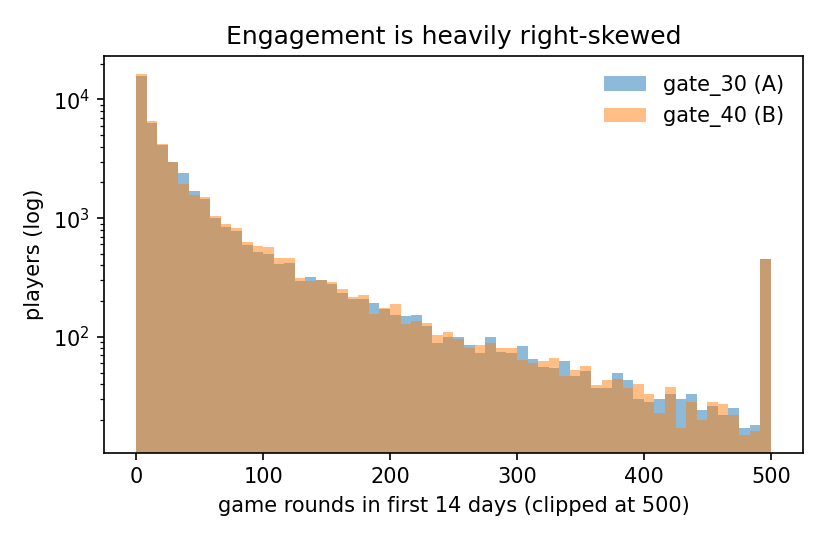
\includegraphics[width=0.48\textwidth]{gamerounds_hist.png}
\caption{Left: 1-day and 7-day retention by version with 95\% normal intervals. Right: distribution of
game rounds (log scale), showing the heavy right skew.}
\end{figure}


\subsection{Checking and cleaning the data}\label{sec:cleaning}
Script: \texttt{src/run\_real.py}.
\begin{enumerate}[nosep]
\item Rows read: \realRaw. Missing entries: \realMissing.
\item Duplicate users: \realUnique{} unique \texttt{userid} values, so \realDup{} duplicate rows.
\item Users in both groups: \realBoth.
\item Rows removed in total: \realRemoved. Rows kept: \realClean.
\item Group sizes: $n_A=\realNA$, $n_B=\realNB$; ratio $n_A/n_B=\realRatio$ (share of $A$: \realShareA).
\item Transformations: \texttt{retention\_1} and \texttt{retention\_7} (True/False) are used as $Y_i=1/0$; nothing else is changed.
\item Train/test split: none. The method estimates two rates and predicts nothing.
\end{enumerate}

% =====================================================================
\section{Method}\label{sec:method}

For one outcome (1-day or 7-day retention) the data reduce to four counts: $n_A$, $n_B$ players and $x_A$, $x_B$
of them who came back (\S\ref{sec:data-math}). The method has five parts; each is derived in
Appendix~\ref{sec:appendix-math}.
\begin{enumerate}[nosep]
\item \textbf{Likelihood.} If players are independent and each comes back with probability $p_v$, the number who
  come back is $X_v\sim\Bin(n_v,p_v)$, so $L(p\mid x)=\binom nx p^x(1-p)^{n-x}$ (Theorem~\ref{thm:binom}).
\item \textbf{Prior and posterior.} With a $\Betad(a,b)$ prior the posterior is
  $p_v\mid\data\sim\Betad(a+x_v,\;b+n_v-x_v)$ (Theorem~\ref{thm:conj}). We use $a=b=1$, the flat prior: every rate
  from 0 to 1 is equally likely before the data. Updating is counting: add the players who came back to $a$ and the
  ones who did not to $b$.
\item \textbf{Posterior summaries.} The posterior mean is a weighted average of the prior mean and the observed
  share, with weight $w=n/(a+b+n)$ on the data, and the posterior variance shrinks as $n$ grows
  (Theorem~\ref{thm:mean}).
\item \textbf{The probability that $B$ is better.} $\theta=\Pr(p_B>p_A\mid\data)=\int_0^1 f_B(t)F_A(t)\,dt$
  (Proposition~\ref{prop:theta}). We estimate it by Monte Carlo with a standard error (Theorem~\ref{thm:mc}) and,
  as a check, by numerical integration. The same posterior draws give a 95\% interval for $p_B-p_A$: the 2.5\% and
  97.5\% quantiles of $p_B^{(m)}-p_A^{(m)}$.
\item \textbf{Frequentist comparison.} The two-proportion $z$ statistic and its two-sided $p$-value
  (Theorem~\ref{thm:z}).
\end{enumerate}
The assumptions behind each part are stated in \S\ref{sec:assumptions} and checked in \S\ref{sec:it3-assump}.

% =====================================================================
\subsection{The algorithm as math}\label{sec:algorithm}

\noindent\textbf{Input:} counts $n_A,x_A,n_B,x_B\in\mathbb N$; prior $a,b>0$; number of draws $M$; level $\alpha$.
\textbf{Output:} posterior parameters, posterior means/variances, $\hat\theta_M$ with SE, and $(z,\,p\text{-value})$.

\begin{enumerate}[leftmargin=*]
\item \textbf{Posterior update} (Theorem~\ref{thm:conj}):
  $\alpha_A=a+x_A$, $\beta_A=b+n_A-x_A$, $\alpha_B=a+x_B$, $\beta_B=b+n_B-x_B$.
  \hfill Sizes: 4 scalars. Operations: 4 additions/subtractions, $O(1)$.
\item \textbf{Posterior summaries} (Theorem~\ref{thm:mean}): for $v\in\{A,B\}$,
  $\mu_v=\alpha_v/(\alpha_v+\beta_v)$, $\sigma_v^2=\alpha_v\beta_v/\big((\alpha_v+\beta_v)^2(\alpha_v+\beta_v+1)\big)$.
  \hfill $O(1)$ (about 12 flops).
\item \textbf{Draw from the posteriors:} $p_A^{(m)}\sim\Betad(\alpha_A,\beta_A)$,
  $p_B^{(m)}\sim\Betad(\alpha_B,\beta_B)$ independently for $m=1,\dots,M$
  (each Beta draw is $G_1/(G_1+G_2)$ with $G_1\sim\Gamma(\alpha,1)$, $G_2\sim\Gamma(\beta,1)$).
  \hfill Sizes: two vectors $\mathbf p_A,\mathbf p_B\in[0,1]^M$. Operations: $2M$ draws, $O(M)$ expected time.
\item \textbf{Indicators and average} (Theorem~\ref{thm:mc}):
  $I_m=\ind{p_B^{(m)}>p_A^{(m)}}$, $\hat\theta_M=\frac1M\sum_{m=1}^M I_m$.
  \hfill $M$ comparisons, $M-1$ additions, 1 division: $O(M)$.
\item \textbf{Standard error:} $\widehat{\mathrm{SE}}=\sqrt{\hat\theta_M(1-\hat\theta_M)/M}$.
  \hfill $O(1)$.
\item \textbf{Frequentist comparison} (Theorem~\ref{thm:z}):
  $\hat p=\frac{x_A+x_B}{n_A+n_B}$,
  $z=\dfrac{x_B/n_B-x_A/n_A}{\sqrt{\hat p(1-\hat p)(1/n_A+1/n_B)}}$,
  $p\text{-value}=2(1-\Phi(|z|))$; reject $H_0$ if $p\text{-value}<\alpha$.
  \hfill $O(1)$ plus one evaluation of $\Phi$.
\item \textbf{Decision:} report $\hat\theta_M\pm\widehat{\mathrm{SE}}$; declare $B$ better if $\hat\theta_M$ exceeds a
  chosen threshold (e.g.\ $0.95$), alongside the $z$ test.
\end{enumerate}
\noindent\textbf{Totals:} time $O(M)$ (dominated by Step~3), memory $O(M)$ for the two draw vectors, or $O(1)$ if the
sum in Step~4 is accumulated on the fly. The data enter only through four integers, so the cost does not grow with
the number of players.

% =====================================================================
\section{From-scratch implementation}\label{sec:impl}

Each step of \S\ref{sec:algorithm} is one function in \texttt{src/methods.py}, written with NumPy only; the comment
above each function is the equation in the table. The same functions run the small example, the simulation and
the real data. \texttt{math.lgamma} and \texttt{math.erfc} (Python standard library) supply $\log\Gamma$ and the
normal tail. SciPy appears only in the check scripts.

\begin{center}\small
\begin{tabular}{l l p{7.6cm}}\toprule
Step & function & equation\\ \midrule
1 & \texttt{my\_posterior} & $\alpha=a+x$, $\beta=b+n-x$ \hfill (Thm.~\ref{thm:conj})\\
2 & \texttt{my\_post\_mean\_var} & $\mu=\frac{\alpha}{\alpha+\beta}$, $\sigma^2=\frac{\alpha\beta}{(\alpha+\beta)^2(\alpha+\beta+1)}$ \hfill (Thm.~\ref{thm:mean})\\
2 & \texttt{my\_weighted\_mean} & $(1-w)\frac a{a+b}+w\frac xn$, $w=\frac n{a+b+n}$ \hfill (Thm.~\ref{thm:mean})\\
3 & \texttt{my\_beta\_draws} & $p^{(m)}=G_1/(G_1+G_2)$, $G_1\sim\Gamma(\alpha,1)$, $G_2\sim\Gamma(\beta,1)$\\
4 & \texttt{my\_indicator\_mean} & $\hat\theta_M=\frac1M\sum_m\ind{p_B^{(m)}>p_A^{(m)}}$ \hfill (Thm.~\ref{thm:mc})\\
5 & \texttt{my\_mc\_se} & $\widehat{\mathrm{SE}}=\sqrt{\hat\theta_M(1-\hat\theta_M)/M}$ \hfill (Thm.~\ref{thm:mc})\\
3--5 & \texttt{my\_mc\_prob} & Steps 3--5 together; returns $(\hat\theta_M,\widehat{\mathrm{SE}})$\\
6 & \texttt{my\_z\_stat} & $z=\frac{x_B/n_B-x_A/n_A}{\sqrt{\hat p(1-\hat p)(1/n_A+1/n_B)}}$, $\hat p=\frac{x_A+x_B}{n_A+n_B}$ \hfill (Thm.~\ref{thm:z})\\
6 & \texttt{my\_p\_value} & $2(1-\Phi(|z|))=\operatorname{erfc}(|z|/\sqrt2)$ \hfill (Thm.~\ref{thm:z})\\
7 & \texttt{my\_decision} & $\hat\theta_M>0.95$; $p\text{-value}<\alpha$\\ \midrule
-- & \texttt{my\_beta\_pdf} & $f(p)=p^{\alpha-1}(1-p)^{\beta-1}/\Bfun(\alpha,\beta)$, computed in logs\\
-- & \texttt{my\_simpson}, \texttt{my\_cumsimpson} & $\int y\approx\frac h3(y_0+4y_1+2y_2+\dots+4y_{N-1}+y_N)$ and its running version\\
-- & \texttt{my\_grid\_prob} & $\theta=\int_0^1 f_B(t)F_A(t)\,dt$ \hfill (Prop.~\ref{prop:theta})\\
-- & \texttt{my\_check\_users}, \texttt{my\_counts} & data check; $n_v=\#\{\text{rows in }v\}$, $x_v=\sum_{i\in v}Y_i$ \hfill (\S\ref{sec:data-math})\\
\bottomrule\end{tabular}\normalsize
\end{center}

\textbf{Grid.} The grid for Proposition~\ref{prop:theta} covers the part of $[0,1]$ within 12 posterior standard
deviations of either posterior mean (for the small example this is all of $[0,1]$). This keeps 2000 intervals
accurate when the posteriors are very narrow, as on the real data where $\sigma\approx0.002$.

\sloppy
\textbf{Simulation code.} \texttt{src/simulate.py} holds the simulation model of Appendix~\ref{sec:sim} as functions:
\texttt{simulate\_ab(pA, pB, n, seed)} returns $(x_A,x_B,n)$, \texttt{simulate\_ab\_many} repeats the experiment,
and \texttt{simulate\_ab\_users} / \texttt{simulate\_overlap\_many} produce the stress-test data in which some
users are in both groups.\par\fussy

% =====================================================================
\section{Verification}\label{sec:verification}

The code is checked three ways before it is trusted on the real data: on a small example small enough to solve by
hand, on simulated data whose true rates we chose, and against SciPy.

\subsection{Hand-worked example}\label{sec:small-summary}
Version $A$: 3 of 10 players come back; version $B$: 5 of 10. The full calculation is in
Appendix~\ref{sec:small}. With the flat prior the posteriors are $\Betad(4,8)$ and $\Betad(6,6)$, with means
$\frac13$ and $\frac12$. Because both densities are polynomials, $\theta$ can be found exactly with fractions:
$\theta=\smThetaExact\approx\smThetaExactDec$. The code's Monte Carlo estimate is $\smThetaMC\pm\smSE$, which is
$\smNSE$ standard errors from the exact value, and its numerical integration on 2000 intervals is within
$\smGridErr$ of it. The $z$ test gives $z=\smZ$ and $p$-value $\smP$. Both methods say the same thing: $B$ looks
better, but 10 players per version are too few to be sure.

% =====================================================================
\subsection{Simulation test: recover the known truth}\label{sec:it3-sim}

Script: \texttt{src/check\_simulation.py}. Data: the simulated experiment of Appendix~\ref{sec:sim} ($p_A=0.10$, $p_B=0.12$, $n=\simn$ per version, seed 0), which gave $x_A=\simxA$, $x_B=\simxB$.

\subsubsection{Comparison with a library}
\begin{itemize}[nosep]
\item $\theta$ on the grid is $\simThetaGrid$; \texttt{scipy.integrate.quad} gives $\simThetaLib$. Difference $\simGridErr$
  (pass criterion $10^{-6}$).
\item The Monte Carlo estimate is $\hat\theta_M=\simThetaMC\pm\simSE$, which is $\simNSE$ standard errors from the
  \texttt{quad} value (pass criterion: below 3).
\item Posterior means and variances against \texttt{scipy.stats.beta}: max difference $\simMomErr$. Our Beta density
  against SciPy's on the whole grid: relative error $\simPdfErr$.
\item $z=\simZ$, $p$-value $\simP$. SciPy has no two-proportion $z$ function, but $z^2$ equals Pearson's chi-square
  statistic of the $2\times2$ table of clicks and non-clicks; against \texttt{chi2\_contingency} (no continuity
  correction) the difference in $z^2$ is $\simZErr$ and in the $p$-value $\simPErr$.
\end{itemize}
\emph{Why the differences have these sizes.} The mean, variance and $z$ are closed formulas, so we and the library
do the same arithmetic and agree to the last bit or to rounding ($10^{-16}$). The grid and \texttt{quad} are two
different approximations of one integral, so they agree to the accuracy of the quadrature ($10^{-12}$). The Monte
Carlo value is a random estimate, so it agrees only to its standard error ($4\times10^{-4}$); that is sampling
error, not rounding. There is no sign or scaling convention to fix except the direction: $\theta$ is
$\Pr(p_B>p_A)$, $z$ is positive when $B$ is ahead, and chi-square loses the sign, which is why $z^2$ is compared.

\subsubsection{Comparison with the truth}
With $n=\simn$: $\mu_A=\simMuA$ (sd $\simSdA$) and $\mu_B=\simMuB$ (sd $\simSdB$) against the true $0.10$ and $0.12$;
$\|(\mu_A,\mu_B)-(p_A,p_B)\|_2=\simTruthErr$, and the larger error is $\simTruthSE$ posterior standard deviations.
Table~\ref{tab:truth} repeats this for four sample sizes. Every single-run error is within 3 standard errors, and
the root-mean-square error over 2000 repetitions follows $\sqrt{p(1-p)/n}$: on log--log axes the slopes are
$\simSlopeA$ and $\simSlopeB$ (theory $-\frac12$), Figure~\ref{fig:errn}.

% Generated by src/check_simulation.py -- do not edit by hand
\begin{table}[ht]\centering
\caption{Simulation against the truth ($p_A=0.10$, $p_B=0.12$). One run per $n$ (seed 0): error of the posterior mean in absolute value and in posterior standard deviations. RMSE over 2000 repetitions against the theoretical $\sqrt{p_A(1-p_A)/n}$.}\label{tab:truth}
\small\begin{tabular}{rrrrrrrrr}\toprule
$n$ & $x_A$ & $x_B$ & $|\mu_A-p_A|$ & in SE & $|\mu_B-p_B|$ & in SE & RMSE$(\mu_A)$ & $\sqrt{p_A(1-p_A)/n}$\\ \midrule
50 & 6 & 5 & 0.03462 & 0.74 & 0.00462 & 0.11 & 0.04338 & 0.04243\\
500 & 51 & 70 & 0.00359 & 0.26 & 0.02143 & 1.38 & 0.01345 & 0.01342\\
5{,}000 & 527 & 602 & 0.00556 & 1.28 & 0.00055 & 0.12 & 0.00428 & 0.00424\\
50{,}000 & 5{,}083 & 6{,}006 & 0.00168 & 1.24 & 0.00014 & 0.09 & 0.00135 & 0.00134\\
\bottomrule\end{tabular}\normalsize\end{table}


\begin{figure}[ht]\centering
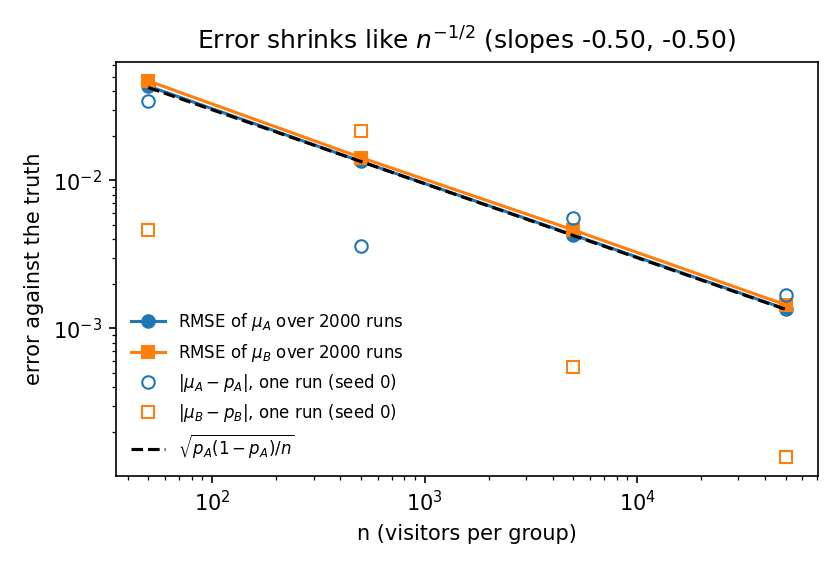
\includegraphics[width=0.6\textwidth]{it3_error_vs_n.png}
\caption{Error of the posterior mean against the true rate, on log--log axes. Filled markers: RMSE over 2000
simulated experiments. Open markers: one experiment (seed 0). Dashed: $\sqrt{p_A(1-p_A)/n}$.}\label{fig:errn}
\end{figure}

\subsubsection{Size of the test}
Repeating the whole experiment 1000 times with $p_A=p_B=0.10$, the $z$ test rejects in $\simNullRej$ of the runs
(pass criterion $0.05\pm0.014$); $z$ has mean $\simNullZmean$ and standard deviation $\simNullZsd$ (theory $0$ and $1$).

\subsubsection{Stress test: 10\% of the users are in both groups}
\textbf{What is broken.} Assumption~\ref{as:random} (the two samples are independent) and
Assumption~\ref{as:indep} (no player counted twice). Of the $n=1000$ users in each group, a fraction $f=0.10$
(100 users) appears in both. Such a user saw both versions, so their one outcome is drawn with the average rate
$\bar p=(p_A+p_B)/2$ and recorded in both groups.

\textbf{What the math says.} Write $x_A=U_A+S$ and $x_B=U_B+S$, where $S\sim\Bin(fn,\bar p)$ is the shared count
and $U_A\sim\Bin((1-f)n,p_A)$, $U_B\sim\Bin((1-f)n,p_B)$. Then $S$ cancels in the difference:
\begin{gather*}
\hat p_B-\hat p_A=\frac{U_B-U_A}{n},\qquad
\E[\hat p_B-\hat p_A]=(1-f)(p_B-p_A),\\
\Var(\hat p_B-\hat p_A)=(1-f)\,\frac{p_A(1-p_A)+p_B(1-p_B)}{n}.
\end{gather*}
So (i) the estimated difference is pulled towards $0$ by the factor $1-f$; (ii) $x_A$ and $x_B$ are positively
correlated, $\operatorname{Cov}(x_A,x_B)=\Var(S)$, giving correlation $\approx f$; and (iii) the $z$ statistic
divides by a standard deviation that is too large by $1/\sqrt{1-f}$, so under $H_0$ it has standard deviation
$\sqrt{1-f}=0.949$ instead of $1$ and rejects with probability $2(1-\Phi(1.96/\sqrt{1-f}))=\strNullRejTheory$ instead of $0.05$.
The posteriors are also wrong: each treats 1000 rows as 1000 independent trials, and their product treats $p_A$ and $p_B$ as independent.

\textbf{What the simulation shows} (20{,}000 repetitions each):
\begin{center}
\begin{tabular}{lrr}\toprule
quantity & clean & 10\% in both groups\\ \midrule
correlation of $x_A$ and $x_B$ ($H_0$) & $\strCleanCorr$ & $+\strNullCorr$\\
standard deviation of $z$ ($H_0$) & \strCleanNullSdZ & \strNullSdZ\\
rejection rate of the $z$ test ($H_0$) & \strCleanNullRej & \strNullRej\\
mean of $\hat p_B-\hat p_A$ (true difference $0.02$) & \strCleanAltDiff & \strAltDiff\\
power of the $z$ test ($p_B=0.12$) & \strCleanAltPower & \strAltPower\\
\bottomrule\end{tabular}
\end{center}
The test is no longer of size $0.05$, the effect is underestimated by 10\%, and power is lost
(Figure~\ref{fig:stress} shows both effects growing with $f$).

\textbf{The data check finds it.} On one stressed data set \texttt{my\_check\_users} reports $\strRows$ rows,
$\strUnique$ unique users and $\strBoth$ users in both groups (the clean simulation gives $0$). As recorded the
counts are $x_A/n_A=\strXA$ and $x_B/n_B=\strXB$; after removing the shared users they are $\strXAc$ and $\strXBc$,
which are again independent binomial samples.

\begin{figure}[ht]\centering
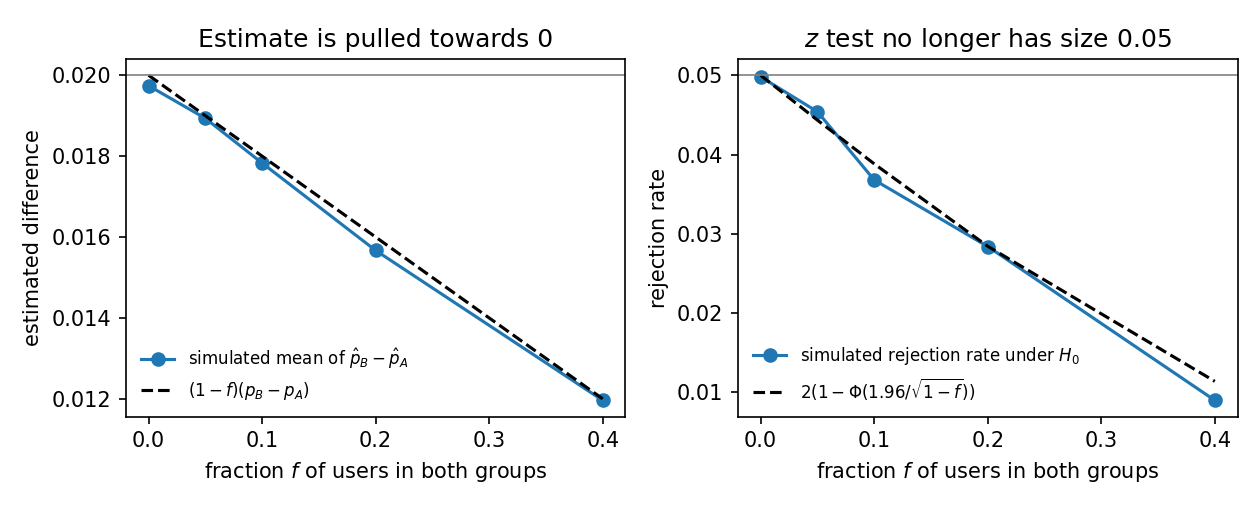
\includegraphics[width=0.85\textwidth]{it3_stress.png}
\caption{Stress test. Left: the estimated difference shrinks like $(1-f)(p_B-p_A)$. Right: the rejection rate of the
$z$ test under $H_0$ falls below $0.05$ as predicted.}\label{fig:stress}
\end{figure}

% =====================================================================
\subsection{Verification table}\label{sec:verif}

Every number is produced by one of the scripts \texttt{small\_example.py}, \texttt{check\_simulation.py}
and \texttt{run\_real.py} in \texttt{src/}.
\begin{center}\small
\resizebox{\textwidth}{!}{%
\begin{tabular}{l l l l c}\toprule
Data & Quantity & Compared with & Difference & Pass?\\ \midrule
\rowsSmall
\midrule
\rowsSim
\midrule
\rowsReal
\bottomrule
\end{tabular}}\normalsize
\end{center}

% =====================================================================
\section{Results on the real data}\label{sec:it3-real}

Script: \texttt{src/run\_real.py}. $A$ = \texttt{gate\_30}, $B$ = \texttt{gate\_40}; a ``click'' is the player returning.

\textbf{Results.} 1-day and 7-day retention are analysed separately (Table~\ref{tab:real}, Figure~\ref{fig:realpost}).
% Generated by src/run_real.py -- do not edit by hand
\begin{table}[ht]\centering
\caption{Cookie Cats, all methods ($n_A=44{,}700$, $n_B=45{,}489$, prior $\Betad(1,1)$, $M=100{,}000$). $\theta=\Pr(p_B>p_A\mid\data)$.}\label{tab:real}
\small\setlength{\tabcolsep}{4pt}\begin{tabular}{lrrrrrrrrr}\toprule
outcome & $x_A$ & $x_B$ & $\mu_A$ & $\mu_B$ & $\sigma_A$ & $\theta$ (grid) & $\hat\theta_M\pm$SE & $z$ & $p$-value\\ \midrule
1-day retention & 20{,}034 & 20{,}119 & 0.4482 & 0.4423 & 0.0024 & 0.03721 & 0.03668 $\pm$ 0.00059 & -1.78 & 0.0744\\
7-day retention & 8{,}502 & 8{,}279 & 0.1902 & 0.1820 & 0.0019 & 0.00078 & 0.00068 $\pm$ 0.00008 & -3.16 & 0.0016\\
\bottomrule\end{tabular}\normalsize\end{table}


\begin{figure}[ht]\centering
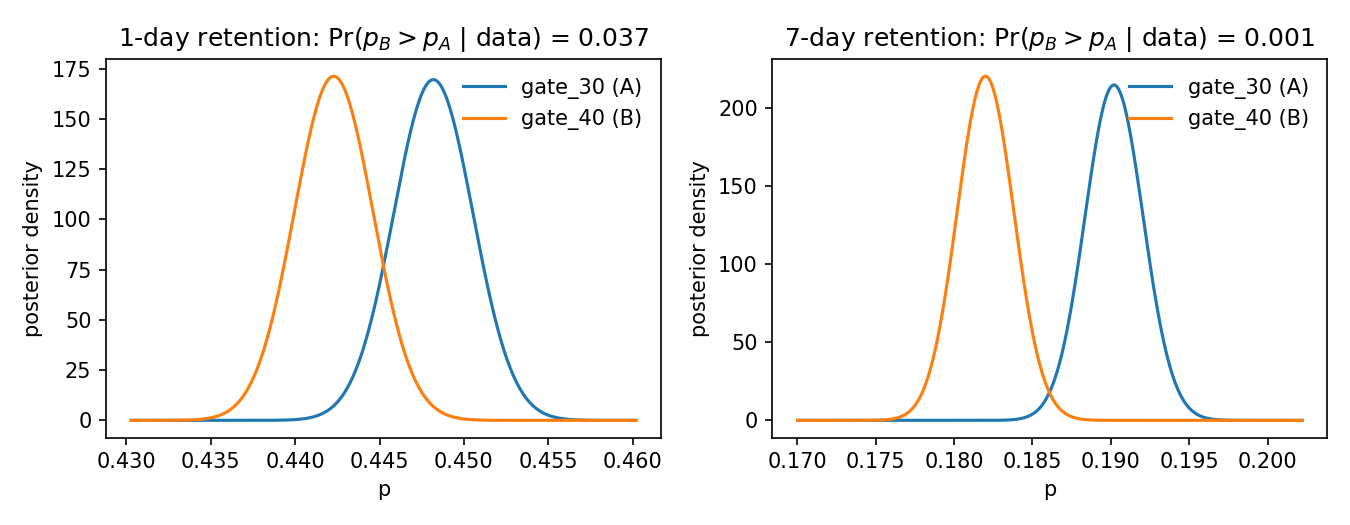
\includegraphics[width=0.9\textwidth]{it3_real_posteriors.png}
\caption{Posterior densities of the retention rates on the real data.}\label{fig:realpost}
\end{figure}

\begin{itemize}[nosep]
\item \emph{7-day retention.} $x_A/n_A=\realSevenRateA$, $x_B/n_B=\realSevenRateB$.
  $\Pr(p_B>p_A\mid\data)=\realSevenThetaFive$, so $\Pr(p_A>p_B\mid\data)=\realSevenThetaA$: moving the gate to level 40
  almost certainly lowers 7-day retention. The posterior mean of $p_B-p_A$ is $\realSevenDiff$ with 95\% interval
  $[\realSevenLo,\ \realSevenHi]$. The $z$ test agrees: $z=\realSevenZ$, $p=\realSevenP$, $H_0$ rejected.
\item \emph{1-day retention.} $x_A/n_A=\realOneRateA$, $x_B/n_B=\realOneRateB$.
  $\Pr(p_A>p_B\mid\data)=\realOneThetaA$; the difference is $\realOneDiff$ with 95\% interval $[\realOneLo,\ \realOneHi]$,
  which contains $0$. The $z$ test gives $z=\realOneZ$, $p=\realOneP$ and does not reject at $\alpha=0.05$.
  The evidence points the same way as for 7 days but is weaker: the Bayesian rule ($\Pr>0.95$) already favours
  $A$, while the two-sided test at $0.05$ does not reject.
\item \emph{Bayesian and frequentist numbers side by side.} The one-sided $p$-value $\Phi(z)$ is $\realOnePhalf$ (1-day)
  and $\realSevenPhalf$ (7-day); $\Pr(p_B>p_A\mid\data)$ is $\realOneThetaFive$ and $\realSevenThetaFive$. With
  $n\approx45{,}000$ the prior has almost no weight and both posteriors are nearly normal, so the two numbers nearly
  coincide, unlike in the small example.
\end{itemize}

\par\noindent\begin{minipage}{\textwidth}\textbf{Library comparison.}
\begin{center}\small
\begin{tabular}{llll}\toprule
quantity & compared with & 1-day & 7-day\\ \midrule
$\mu_A,\mu_B,\sigma_A^2,\sigma_B^2$ & \texttt{scipy.stats.beta} & max$|\cdot|=\realOneMomErr$ & max$|\cdot|=\realSevenMomErr$\\
Beta density on the grid & \texttt{stats.beta.pdf} & rel.\ $\realOnePdfErr$ & rel.\ $\realSevenPdfErr$\\
$\theta$ (grid) & \texttt{integrate.quad} & $\realOneGridErr$ & $\realSevenGridErr$\\
$\hat\theta_M$ & \texttt{integrate.quad} & \realOneNSE{} SE & \realSevenNSE{} SE\\
$z^2$ & \texttt{chi2\_contingency} & rel.\ $\realOneZErr$ & rel.\ $\realSevenZErr$\\
$p$-value & \texttt{chi2\_contingency} & $\realOnePErr$ & $\realSevenPErr$\\
\bottomrule\end{tabular}\normalsize
\end{center}\end{minipage}

\emph{Size of the differences.} As in the simulation: closed formulas agree to rounding; $z^2$ is now about $10$ and
is built from counts near $20{,}000$, so its rounding error is $10^{-14}$ rather than $0$; the density differs in the
11th digit because we compute $\log\Bfun$ with \texttt{lgamma} of arguments near $45{,}000$, where each
$\log\Gamma$ is about $4\times10^5$ and the subtraction loses digits; the grid and \texttt{quad} agree to $10^{-12}$;
Monte Carlo agrees to about one standard error. For 7-day retention $\theta$ is tiny, so although the absolute
Monte Carlo error is small ($\widehat{\mathrm{SE}}=\realSevenSE$), the relative error
$\sqrt{(1-\theta)/(\theta M)}$ is about 11\%; the grid value is the one to quote for a small probability.

\subsection{What the results mean}\label{sec:meaning}

\textbf{7-day retention.} Given the data, the probability that level 30 keeps more players after a week is
$\realSevenThetaA$. The most likely size of the effect is $p_B-p_A=\realSevenDiff$: moving the gate to level 40 costs
about $0.8$ percentage points of 7-day retention, which is about 8 of every 1{,}000 new players. The 95\% interval,
$[\realSevenLo,\ \realSevenHi]$, is about 3 to 13 players per 1{,}000 and does not contain 0. The $z$ test rejects
$H_0$ with $p$-value $\realSevenP$. Both methods point the same way, and the effect is small but clear.

\textbf{1-day retention.} The probability that level 30 is better is $\realOneThetaA$, and the estimated cost of
moving the gate is about 6 players per 1{,}000 ($\realOneDiff$). The 95\% interval $[\realOneLo,\ \realOneHi]$
contains 0, so on its own this result is not conclusive.

\textbf{Why the two methods only seem to disagree on 1-day retention.} The posterior rule ``$\Pr(p_A>p_B\mid\data)>0.95$''
says $A$ is better ($\realOneThetaA$), while the two-sided $z$ test at $0.05$ does not reject ($p$-value $\realOneP$).
The evidence behind the two is the same. With the flat prior and about 45{,}000 players per version, the posteriors
are almost normal and the prior has almost no weight, so $\Pr(p_B>p_A\mid\data)$ almost equals the one-sided
$p$-value $\Phi(z)$: $\realOneThetaFive$ against $\realOnePhalf$. The two rules draw the line in different places: the
posterior rule asks for this number to be below $0.05$, and the two-sided test at $0.05$ asks for it to be below
$0.025$. The 1-day value lies between the two cutoffs. The threshold $0.95$ is a convention, not a law.

\textbf{Which number to quote.} For 7-day retention $\theta$ is very small, so the Monte Carlo estimate has a large
relative error even with $M=100{,}000$ draws (\S\ref{sec:it3-real}); the numerical-integration value is the one we
quote.

% =====================================================================
\section{Assumptions and limitations}\label{sec:limits}

% =====================================================================
\subsection{The assumptions}\label{sec:assumptions}

\begin{assumption}[Bernoulli outcomes with a common rate within a version]\label{as:bern}
Within version $A$ every player clicks with the same probability $p_A$ (and likewise $p_B$).\\
\emph{If it fails:} $X_A$ is not $\Bin(n_A,p_A)$; the true variance of $X_A$ is larger than $n_Ap_A(1-p_A)$
(over-dispersion), so posteriors and the $z$ test are too confident.\\
\emph{Check (\S\ref{sec:it3-assump}):} split each version into random batches and compare the batch-to-batch
variance of the rate with $\hat p(1-\hat p)/n_{\text{batch}}$; compare rates across strata of
\texttt{sum\_gamerounds}.
\end{assumption}

\begin{assumption}[Independent trials]\label{as:indep}
Outcomes of different players are independent.\\
\emph{If it fails:} the product rule in Theorem~\ref{thm:binom} does not hold, the likelihood is wrong,
and $\Var(\hat p)=p(1-p)/n$ (used in Theorem~\ref{thm:z}) is wrong.\\
\emph{Check:} confirm \texttt{userid} is unique (no player counted twice) and that there is no
obvious clustering (e.g.\ by install date, if available).
\end{assumption}

\begin{assumption}[Randomised assignment; $A$ and $B$ independent]\label{as:random}
Version is assigned at random, so the two samples are independent and $p_A$, $p_B$ have independent
posteriors.\\
\emph{If it fails:} $\Pr(p_B>p_A\mid\data)$ can no longer be computed from the product of the two
posteriors (Theorem~\ref{thm:mc}), and any difference may be confounding rather than the gate.\\
\emph{Check:} compare the group sizes with what a fair coin would give (binomial test on $n_A$ vs
$n_A+n_B$); compare the distribution of pre-gate behaviour (rounds played below level 30) across versions.
\end{assumption}

\begin{assumption}[Beta prior with $a,b>0$, chosen before seeing the data]\label{as:prior}
\emph{If it fails:} with $a\le0$ or $b\le0$ the prior does not integrate; with a non-Beta prior the
posterior is not Beta and must be computed numerically.\\
\emph{Check:} repeat the analysis with $\Betad(1,1)$, $\Betad(0.5,0.5)$ and $\Betad(2,2)$ and report the
change in $\theta$ (prior sensitivity); with $n\approx45{,}000$ the weight $w=n/(a+b+n)$ is $\approx1$, so the
prior should matter very little.
\end{assumption}

\begin{assumption}[Large samples for the normal approximation]\label{as:clt}
$n_Ap_A$, $n_A(1-p_A)$, $n_Bp_B$, $n_B(1-p_B)$ are all large (rule of thumb $\ge10$).\\
\emph{If it fails:} $z$ is not approximately $N(0,1)$ under $H_0$, so the test does not have size $\alpha$.\\
\emph{Check:} compute $n\hat p$ and $n(1-\hat p)$ on the data (they are in the thousands), and
compare the rejection rate under a simulated null with $\alpha$ (done in \S\ref{sec:sim}).
\end{assumption}

\begin{assumption}[I.i.d.\ Monte Carlo draws]\label{as:mc}
The $M$ posterior draws are independent and come exactly from the Beta posteriors.\\
\emph{If it fails:} $\hat\theta_M$ may be biased and the standard error $\sqrt{\theta(1-\theta)/M}$ is wrong.\\
\emph{Check:} the empirical standard deviation of $\hat\theta_M$ over repeated runs should fall like
$M^{-1/2}$ (Figure~\ref{fig:mcse}); results should not change with the seed beyond the SE.
\end{assumption}

\begin{assumption}[No missing or corrupted outcomes]\label{as:missing}
Every player has a recorded version and retention value.\\
\emph{If it fails:} $n$ and $x$ are miscounted, and missingness that depends on the outcome biases $\hat p$.\\
\emph{Check:} count missing values per column (\S\ref{sec:data}) and inspect extreme
\texttt{sum\_gamerounds} values.
\end{assumption}

% =====================================================================
\subsection{Checking the assumptions}\label{sec:it3-assump}

Script: \texttt{src/check\_assumptions.py}. Each check is run first on simulated data (the model of Appendix~\ref{sec:sim}, 2000
users assigned to $A$ or $B$ by a fair coin), where the assumption holds by construction, and then on Cookie Cats.
Batches are consecutive blocks of rows in file order, which is increasing \texttt{userid}.

\begin{center}\small
\begin{tabular}{p{3.2cm} p{3.2cm} p{2.6cm} p{2.6cm} p{2.6cm}}\toprule
Assumption & check & simulated & real, 1-day & real, 7-day\\ \midrule
\ref{as:bern} common rate & $\chi^2_9$ over 10 batches: $A$; $B$ ($p$-values) &
  \asSimXA{} (\asSimXAp); \asSimXB{} (\asSimXBp) & \asOneXA{} (\asOneXAp); \asOneXB{} (\asOneXBp) & \asSevenXA{} (\asSevenXAp); \asSevenXB{} (\asSevenXBp)\\
\ref{as:indep} independence & duplicate rows; lag-1 autocorrelation $A$, $B$ ($z$) &
  \asSimDup; $\asSimRA$ ($\asSimRAz$), $\asSimRB$ ($\asSimRBz$) & \asOneDup; $\asOneRA$ ($\asOneRAz$), $\asOneRB$ ($\asOneRBz$) &
  \asSevenDup; $\asSevenRA$ ($\asSevenRAz$), $\asSevenRB$ ($\asSevenRBz$)\\
\ref{as:random} randomised groups & users in both groups; $z$ for a 50/50 split ($p$) &
  \asSimBoth; $\asSimSplitZ$ (\asSimSplitP) & \asOneBoth; $\asOneSplitZ$ (\asOneSplitP) & same groups\\
\ref{as:prior} prior & range of $\theta$ over three priors & $\asSimPriorRange$ & $\asOnePriorRange$ & $\asSevenPriorRange$\\
\ref{as:clt} large samples & smallest of $n\hat p$, $n(1-\hat p)$ & \asSimSmallest & \asOneSmallest & \asSevenSmallest\\
\ref{as:mc} i.i.d.\ draws & sd of $\hat\theta_M$ over 30 seeds / SE formula & \asSimMcRatio & \asOneMcRatio & \asSevenMcRatio\\
\ref{as:missing} no missing & missing entries & 0 & \asMissing & \asMissing\\
\bottomrule\end{tabular}\normalsize
\end{center}

\textbf{What we found.}
\begin{itemize}[nosep]
\item \emph{Assumption~\ref{as:bern} (common rate).} On the real data the batch-to-batch variation of the rate is
  what a binomial predicts (all four $p$-values are large). On the simulated data set the check for group $A$ gave
  $p=\asSimXAp$ although the assumption is true there. This is a false alarm: over 500 simulated data sets the same
  check gives $p<0.05$ in $\asSimAlarm$ of them, close to the $0.05$ it should. So a single small $p$-value from this
  check is not proof of a problem, and a ``pass'' means a $p$-value that is not small.
  Players are certainly not identical: 7-day retention is $\asStrataLow$ in the lowest quartile of
  \texttt{sum\_gamerounds} and $\asStrataHigh$ in the highest. This does not break the binomial model, because each
  player is a random draw from the population of players, so $\Pr(Y_i=1)=\E[p_i]=p_A$ for every row.
\item \emph{Assumption~\ref{as:indep} (independence).} No \texttt{userid} is repeated, and neighbouring rows are
  uncorrelated ($|z|<2$ in every case).
\item \emph{Assumption~\ref{as:random} (randomisation).} No user is in both groups. The group sizes, however, are
  $\asOneNA$ and $\asOneNB$: under a fair coin $n_A$ would be $\Bin(N,\frac12)$, and the observed split is
  $z=\asOneSplitZ$ ($p=\asOneSplitP$) from 50/50. The simulated split gives $z=\asSimSplitZ$. This is a sample-ratio
  mismatch: group $A$ has $\realFewer\%$ fewer players than group $B$. The method does not need equal group sizes, but it does need assignment to be unrelated
  to the outcome, and an unexplained imbalance is a warning that it may not be (for example, players lost from one
  group before being logged). We cannot test this further with the columns available; pre-gate behaviour is similar
  (median rounds \asMedA{} and \asMedB, share with zero rounds \asZeroA{} and \asZeroB). We report it as a caveat.
\item \emph{Assumption~\ref{as:prior} (prior).} $\theta$ changes by less than $10^{-5}$ between $\Betad(1,1)$,
  $\Betad(\frac12,\frac12)$ and $\Betad(2,2)$ on the real data, because $w=\asOneW$.
\item \emph{Assumption~\ref{as:clt} (large samples).} $n\hat p$ and $n(1-\hat p)$ are in the thousands on the real
  data (and above 100 in the simulation), far above 10. In the small example they are 4 and 6, which is why the
  normal approximation was only rough there.
\item \emph{Assumption~\ref{as:mc} (Monte Carlo draws).} Over 30 seeds the standard deviation of $\hat\theta_M$
  matches $\sqrt{\theta(1-\theta)/M}$ (ratios near 1).
\item \emph{Assumption~\ref{as:missing} (missing values).} There are \asMissing{} missing entries. One player has
  \asMaxRounds{} game rounds, an outlier, but \texttt{sum\_gamerounds} is not used by the method.
\end{itemize}

\subsection{Limitations}\label{sec:limitations}
\begin{itemize}[nosep]
\item \textbf{Uneven group sizes.} Group $A$ has $\realFewer\%$ fewer players than group $B$, which a fair coin
  would rarely give ($p$-value \asOneSplitP). The method does not need equal groups, but it does need assignment to
  be unrelated to whether players come back. The available columns cannot explain the imbalance, so the results
  depend on it being harmless.
\item \textbf{Players in both groups.} None are present here, but the stress test (\S\ref{sec:it3-sim}) shows what
  they would do: the estimated difference shrinks by the share of such players and the $z$ test loses power.
\item \textbf{One outcome at a time.} 1-day and 7-day retention are analysed separately, and they come from the
  same players, so they are not two independent pieces of evidence.
\item \textbf{Retention only.} The report measures whether players come back, not how much they play
  (\texttt{sum\_gamerounds} is used only in the checks).
\item \textbf{One experiment.} The results describe this game and these players; they say nothing directly about
  gates in other games.
\end{itemize}

% =====================================================================
\section{Conclusion}\label{sec:conclusion}
Moving the Cookie Cats gate from level 30 to level 40 lowers 7-day retention. The probability that level 30 keeps
more players is $\realSevenThetaA$, the estimated loss is about 8 of every 1{,}000 players with a 95\% interval of
about 3 to 13, and the $z$ test agrees ($p$-value $\realSevenP$). 1-day retention points the same way with weaker
evidence. \textbf{We recommend keeping the gate at level 30.}

The answer rests on a short chain of results derived by hand: the binomial likelihood, Beta--binomial conjugacy,
the posterior mean and variance, the Monte Carlo estimator and its standard error, and the two-proportion $z$
statistic. The from-scratch code reproduces the exact hand-worked answer, recovers the known truth in simulation,
and agrees with SciPy on the real data. The main caveat is the unexplained imbalance in group sizes; checking how
players were assigned and logged would be the first step before acting on the result.

% =====================================================================
\clearpage
\appendix
\section{Mathematical appendix}\label{sec:appendix-math}
This appendix holds all notation, definitions and derivations, the hand-worked example, and the answers to the
math questions of Iterations 2 and 3.

% =====================================================================
\subsection{Notation}\label{sec:notation}

\begin{center}
\small\begin{tabular}{>{$}l<{$} p{7.4cm} l}\toprule
\text{Symbol} & Meaning & Dimension / set\\ \midrule
A,\;B & the two versions (control, treatment) & labels\\
n_A,\,n_B & number of visitors (trials) shown version $A$, $B$ & $\mathbb N$\\
Y_{A,i} & outcome of visitor $i$ in version $A$: $1$ = click, $0$ = no click & $\{0,1\}$\\
x_A,\,x_B & number of clicks, $x_A=\sum_{i=1}^{n_A}Y_{A,i}$ & $\{0,1,\dots,n\}$\\
X_A,\,X_B & the click counts seen as random variables & $\Bin(n_A,p_A)$, $\Bin(n_B,p_B)$\\
p_A,\,p_B & true (unknown) click probabilities & $[0,1]$\\
\hat p_A,\,\hat p_B & observed rates $x_A/n_A$, $x_B/n_B$ & $[0,1]$\\
\binom{n}{x} & binomial coefficient $n!/(x!(n-x)!)$ & $\mathbb N$\\
L(p\mid x) & likelihood of $p$ given $x$ clicks in $n$ trials & $[0,1]$\\
a,\,b & prior parameters of $\Betad(a,b)$ (we use $a=b=1$) & $(0,\infty)$\\
\pi(p),\;\pi(p\mid x) & prior and posterior density of $p$ & densities on $[0,1]$\\
m(x) & marginal (prior predictive) probability of $x$ & $[0,1]$\\
\Gamma(\cdot),\;\Bfun(\cdot,\cdot) & Gamma function, Beta function & $(0,\infty)$\\
\alpha_A,\beta_A & posterior parameters $a+x_A$, $b+n_A-x_A$ & $(0,\infty)$\\
w & weight on the data in the posterior mean, $n/(a+b+n)$ & $(0,1)$\\
\theta & $\Pr(p_B>p_A\mid\data)$, the quantity we report & $[0,1]$\\
M & number of Monte Carlo draws & $\mathbb N$\\
p_A^{(m)},\,p_B^{(m)} & $m$-th posterior draw, $m=1,\dots,M$ & $[0,1]$\\
I_m & indicator $\ind{p_B^{(m)}>p_A^{(m)}}$ & $\{0,1\}$\\
\hat\theta_M & Monte Carlo estimate $\frac1M\sum_m I_m$ & $[0,1]$\\
\mathrm{SE} & standard error (standard deviation of an estimator) & $(0,\infty)$\\
H_0 & null hypothesis $p_A=p_B$ & --\\
\hat p & pooled rate $(x_A+x_B)/(n_A+n_B)$ & $[0,1]$\\
z & two-proportion $z$ statistic & $\mathbb R$\\
\Phi,\;z_{1-\alpha/2} & standard normal CDF and its $(1-\alpha/2)$ quantile & --\\
\alpha & significance level (we use $0.05$); not the posterior parameters $\alpha_A,\alpha_B$ & $(0,1)$\\
\mathbf 1,\;\ind{\cdot} & indicator of an event & $\{0,1\}$\\
\bottomrule
\end{tabular}\normalsize
\end{center}

% =====================================================================
\subsection{Definitions}\label{sec:definitions}

\begin{definition}[Bernoulli trial]
A random variable $Y$ with $\Pr(Y=1)=p$ and $\Pr(Y=0)=1-p$, $p\in[0,1]$, is a
$\Ber(p)$ trial. Its probability mass function can be written $\Pr(Y=y)=p^{y}(1-p)^{1-y}$, $y\in\{0,1\}$.
\end{definition}

\begin{definition}[Independence]
Events $E_1,\dots,E_n$ are mutually independent if
$\Pr(E_{i_1}\cap\cdots\cap E_{i_k})=\prod_{j=1}^k\Pr(E_{i_j})$ for every sub-collection.
Random variables are independent if every collection of events $\{Y_i\in S_i\}$ is independent.
Random variables that are independent and share one distribution are \emph{i.i.d.}
\end{definition}

\begin{definition}[Binomial distribution]
$X\sim\Bin(n,p)$ if $\Pr(X=x)=\binom nx p^x(1-p)^{n-x}$ for $x\in\{0,\dots,n\}$.
(Theorem~\ref{thm:binom} shows this is the distribution of a sum of $n$ i.i.d.\ $\Ber(p)$ trials.)
\end{definition}

\begin{definition}[Conditional probability and Bayes' theorem]
For events with $\Pr(B)>0$, $\Pr(A\mid B)=\Pr(A\cap B)/\Pr(B)$. Hence
$\Pr(A\mid B)=\Pr(B\mid A)\Pr(A)/\Pr(B)$ (Bayes' theorem). For a continuous parameter $p$
with density $\pi(p)$ and an observation $x$ with $\Pr(x\mid p)=L(p\mid x)$, the
\emph{posterior density} is
\[
\pi(p\mid x)=\frac{L(p\mid x)\,\pi(p)}{m(x)},\qquad m(x)=\int_0^1 L(p\mid x)\,\pi(p)\,dp .
\]
$\pi(p)$ is the \emph{prior}, $L(p\mid x)$ the \emph{likelihood} (the probability of the data seen as a
function of $p$), and $m(x)$ the \emph{marginal likelihood}.
\end{definition}

\begin{definition}[Gamma and Beta functions]
$\Gamma(s)=\int_0^\infty t^{s-1}e^{-t}\,dt$ for $s>0$; it satisfies $\Gamma(s+1)=s\Gamma(s)$ and
$\Gamma(k)=(k-1)!$ for integers $k\ge1$. The Beta function is
\[
\Bfun(\alpha,\beta)=\int_0^1 t^{\alpha-1}(1-t)^{\beta-1}\,dt=\frac{\Gamma(\alpha)\Gamma(\beta)}{\Gamma(\alpha+\beta)},
\qquad \alpha,\beta>0 .
\]
\end{definition}

\begin{definition}[Beta distribution]
$p\sim\Betad(\alpha,\beta)$, $\alpha,\beta>0$, if its density on $[0,1]$ is
$f(p)=p^{\alpha-1}(1-p)^{\beta-1}/\Bfun(\alpha,\beta)$. $\Betad(1,1)$ is the uniform distribution.
\end{definition}

\begin{definition}[Conjugate prior]
A family of priors is \emph{conjugate} to a likelihood if, for every prior in the family and every
possible observation, the posterior is again in the family.
\end{definition}

\begin{definition}[Expectation, variance, indicator]
For a discrete $Y$, $\E[Y]=\sum_y y\Pr(Y=y)$; for a continuous $p$ with density $f$, $\E[g(p)]=\int g(p)f(p)\,dp$.
$\Var(Y)=\E[(Y-\E Y)^2]=\E[Y^2]-(\E Y)^2$. The indicator of an event $E$ is $\ind{E}=1$ if $E$
occurs and $0$ otherwise; $\E[\ind{E}]=\Pr(E)$.
\end{definition}

\begin{definition}[Estimator, unbiasedness, standard error]
An estimator $\hat\theta$ of $\theta$ is a function of the data (or of the random draws).
It is \emph{unbiased} if $\E[\hat\theta]=\theta$. Its \emph{standard error} is
$\mathrm{SE}(\hat\theta)=\sqrt{\Var(\hat\theta)}$.
\end{definition}

\begin{definition}[Monte Carlo estimator]
If $\theta=\E[g(Z)]$ and $Z^{(1)},\dots,Z^{(M)}$ are i.i.d.\ copies of $Z$, the Monte Carlo estimator is
$\hat\theta_M=\frac1M\sum_{m=1}^M g(Z^{(m)})$.
\end{definition}

\begin{definition}[Central limit theorem (statement used)]
If $Y_1,\dots,Y_n$ are i.i.d.\ with mean $\mu$ and variance $\sigma^2<\infty$, then
$\sqrt n(\bar Y_n-\mu)/\sigma\to N(0,1)$ in distribution. For $\Ber(p)$ trials
($\mu=p$, $\sigma^2=p(1-p)$) this is the de Moivre--Laplace theorem:
$\hat p=X/n$ is approximately $N\!\big(p,\;p(1-p)/n\big)$ for large $n$.
\end{definition}

\begin{definition}[Hypothesis test, test statistic, $p$-value]
A null hypothesis $H_0$ is a statement about the parameters (here $p_A=p_B$).
A test statistic $T$ is a function of the data whose distribution under $H_0$ is known
(at least approximately). The two-sided $p$-value is $\Pr_{H_0}(|T|\ge|t_{\mathrm{obs}}|)$,
and the test of size $\alpha$ rejects $H_0$ when the $p$-value is below $\alpha$.
\end{definition}

% =====================================================================
\subsection{Derivations}\label{sec:derivations}

\subsubsection{The binomial likelihood (Q1)}

\begin{theorem}[Binomial likelihood]\label{thm:binom}
Let $Y_1,\dots,Y_n$ be i.i.d.\ $\Ber(p)$ and $X=\sum_{i=1}^n Y_i$. Then
\[
\Pr(X=x\mid p)=\binom{n}{x}p^{x}(1-p)^{n-x},\qquad x=0,1,\dots,n,
\]
so the likelihood of $p$ given $x$ clicks in $n$ visits is $L(p\mid x)=\binom nx p^x(1-p)^{n-x}$.
Moreover $L(p\mid x)$ is maximised at $\hat p=x/n$.
\end{theorem}

\begin{proof}
\emph{Step 1 (probability of one particular sequence).}
Fix a sequence $(y_1,\dots,y_n)\in\{0,1\}^n$ with exactly $x$ ones. By independence,
\[
\Pr(Y_1=y_1,\dots,Y_n=y_n)=\prod_{i=1}^n\Pr(Y_i=y_i)=\prod_{i=1}^n p^{y_i}(1-p)^{1-y_i}
= p^{\sum y_i}(1-p)^{n-\sum y_i}=p^{x}(1-p)^{n-x}.
\tag*{[\emph{independence; Bernoulli pmf; laws of exponents}]}
\]
\emph{Step 2 (how many such sequences).}
The number of sequences of length $n$ with exactly $x$ ones is the number of ways to choose the
positions of the ones, $\binom nx$. \rulename{counting / definition of the binomial coefficient}

\emph{Step 3 (add them up).}
The event $\{X=x\}$ is the disjoint union of the $\binom nx$ events ``the sequence equals $(y_1,\dots,y_n)$''
over all sequences with $x$ ones. Probabilities of disjoint events add, and each has the probability from
Step~1, so $\Pr(X=x\mid p)=\binom nx p^x(1-p)^{n-x}$. \rulename{additivity of probability}

\emph{Step 4 (maximiser).}
For $0<x<n$, $\ell(p)=\log L(p\mid x)=\log\binom nx+x\log p+(n-x)\log(1-p)$ and
$\ell'(p)=\frac xp-\frac{n-x}{1-p}$. Setting $\ell'(p)=0$ gives $x(1-p)=(n-x)p$, i.e.\ $p=x/n$.
Since $\ell''(p)=-\frac x{p^2}-\frac{n-x}{(1-p)^2}<0$, this is a maximum. For $x=0$ or $x=n$ the
likelihood is monotone and the maximiser is the endpoint $x/n$.
\rulename{log is increasing; first- and second-order conditions}
\end{proof}

\subsubsection{Beta--binomial conjugacy (Q2)}

\begin{theorem}[Conjugacy]\label{thm:conj}
If $p\sim\Betad(a,b)$ a priori and $X\mid p\sim\Bin(n,p)$, then
\[
p\mid X=x\;\sim\;\Betad(a+x,\;b+n-x).
\]
Hence the Beta family is conjugate to the binomial likelihood, and the marginal likelihood is
$m(x)=\binom nx\,\Bfun(a+x,b+n-x)/\Bfun(a,b)$ (the Beta--binomial pmf).
\end{theorem}

\begin{proof}
\emph{Step 1 (write down Bayes' theorem).}
\[
\pi(p\mid x)=\frac{L(p\mid x)\,\pi(p)}{m(x)},\qquad m(x)=\int_0^1 L(p\mid x)\pi(p)\,dp .
\tag*{[\emph{Bayes' theorem for densities}]}
\]
\emph{Step 2 (multiply likelihood and prior).} By Theorem~\ref{thm:binom} and the Beta density,
\[
L(p\mid x)\,\pi(p)=\binom nx p^x(1-p)^{n-x}\cdot\frac{p^{a-1}(1-p)^{b-1}}{\Bfun(a,b)}
=\frac{\binom nx}{\Bfun(a,b)}\;p^{(a+x)-1}(1-p)^{(b+n-x)-1}.
\tag*{[\emph{Theorem~\ref{thm:binom}; Beta density; add exponents}]}
\]
\emph{Step 3 (normalising constant).} Integrate Step~2 over $p$. Because $a+x>0$ and $b+n-x>0$
the integral is a Beta function:
\[
m(x)=\frac{\binom nx}{\Bfun(a,b)}\int_0^1 p^{(a+x)-1}(1-p)^{(b+n-x)-1}\,dp
=\frac{\binom nx}{\Bfun(a,b)}\,\Bfun(a+x,\,b+n-x).
\tag*{[\emph{definition of the Beta function}]}
\]
\emph{Step 4 (divide).} The constant $\binom nx/\Bfun(a,b)$ cancels:
\[
\pi(p\mid x)=\frac{p^{(a+x)-1}(1-p)^{(b+n-x)-1}}{\Bfun(a+x,\,b+n-x)},
\]
which is exactly the $\Betad(a+x,b+n-x)$ density. \rulename{definition of the Beta distribution}

\emph{Step 5 (conjugacy).} The prior was in the Beta family and so is the posterior, for every
$a,b>0$ and every $x\in\{0,\dots,n\}$; this is the definition of a conjugate family.
\end{proof}

\begin{remark}
The posterior depends on the data only through $x$ and $n$: $a$ acts like $a$ ``prior clicks'' and $b$ like
$b$ ``prior non-clicks''. Applying the theorem to each version separately (Assumption~\ref{as:random}) gives
$p_A\mid\data\sim\Betad(\alpha_A,\beta_A)$ with $\alpha_A=a+x_A$, $\beta_A=b+n_A-x_A$, and similarly for $B$.
\end{remark}

\subsubsection{Posterior mean and variance (Q3)}

\begin{lemma}[Moments of the Beta distribution]\label{lem:moments}
If $p\sim\Betad(\alpha,\beta)$ then for every $k\ge0$,
$\E[p^k]=\Bfun(\alpha+k,\beta)/\Bfun(\alpha,\beta)$. In particular
\[
\E[p]=\frac{\alpha}{\alpha+\beta},\qquad
\E[p^2]=\frac{\alpha(\alpha+1)}{(\alpha+\beta)(\alpha+\beta+1)},\qquad
\Var(p)=\frac{\alpha\beta}{(\alpha+\beta)^2(\alpha+\beta+1)} .
\]
\end{lemma}

\begin{proof}
\emph{Step 1.}
\[
\E[p^k]=\int_0^1 p^k\frac{p^{\alpha-1}(1-p)^{\beta-1}}{\Bfun(\alpha,\beta)}dp
=\frac{1}{\Bfun(\alpha,\beta)}\int_0^1 p^{(\alpha+k)-1}(1-p)^{\beta-1}dp=\frac{\Bfun(\alpha+k,\beta)}{\Bfun(\alpha,\beta)}.
\tag*{[\emph{definition of expectation; definition of the Beta function}]}
\]

\emph{Step 2.} Write both Beta functions with Gamma functions and use $\Gamma(s+1)=s\Gamma(s)$:
\[
\frac{\Bfun(\alpha+1,\beta)}{\Bfun(\alpha,\beta)}
=\frac{\Gamma(\alpha+1)\Gamma(\beta)}{\Gamma(\alpha+\beta+1)}\cdot\frac{\Gamma(\alpha+\beta)}{\Gamma(\alpha)\Gamma(\beta)}
=\frac{\alpha\,\Gamma(\alpha)}{(\alpha+\beta)\Gamma(\alpha+\beta)}\cdot\frac{\Gamma(\alpha+\beta)}{\Gamma(\alpha)}
=\frac{\alpha}{\alpha+\beta}.
\tag*{[\emph{$\Bfun=\Gamma\Gamma/\Gamma$; $\Gamma(s+1)=s\Gamma(s)$}]}
\]
Applying the same identity twice gives $\E[p^2]=\frac{\alpha(\alpha+1)}{(\alpha+\beta)(\alpha+\beta+1)}$.

\emph{Step 3.}
\begin{align*}
\Var(p)&=\E[p^2]-(\E p)^2
=\frac{\alpha(\alpha+1)}{(\alpha+\beta)(\alpha+\beta+1)}-\frac{\alpha^2}{(\alpha+\beta)^2}\\
&=\frac{\alpha(\alpha+1)(\alpha+\beta)-\alpha^2(\alpha+\beta+1)}{(\alpha+\beta)^2(\alpha+\beta+1)}
=\frac{\alpha\beta}{(\alpha+\beta)^2(\alpha+\beta+1)},
\end{align*}
since the numerator simplifies to $\alpha[(\alpha+1)(\alpha+\beta)-\alpha(\alpha+\beta+1)]=\alpha[\alpha+\beta-\alpha]=\alpha\beta$.
\rulename{variance formula; algebra}
\end{proof}

\begin{theorem}[Posterior mean as a weighted average; posterior variance]\label{thm:mean}
Under the model of Theorem~\ref{thm:conj},
\[
\E[p\mid x]=\frac{a+x}{a+b+n}=(1-w)\,\frac{a}{a+b}+w\,\frac{x}{n},
\qquad w=\frac{n}{a+b+n}\in(0,1),
\]
i.e.\ the posterior mean is a convex combination of the prior mean $a/(a+b)$ (weight $1-w=\frac{a+b}{a+b+n}$)
and the observed rate $x/n$ (weight $w$). Furthermore
\[
\Var(p\mid x)=\frac{(a+x)(b+n-x)}{(a+b+n)^2(a+b+n+1)} .
\]
\end{theorem}

\begin{proof}
\emph{Step 1.} By Theorem~\ref{thm:conj} the posterior is $\Betad(\alpha,\beta)$ with $\alpha=a+x$, $\beta=b+n-x$,
so $\alpha+\beta=a+b+n$. \rulename{Theorem~\ref{thm:conj}}

\emph{Step 2.} Lemma~\ref{lem:moments} gives $\E[p\mid x]=\frac{a+x}{a+b+n}$ and
$\Var(p\mid x)=\frac{(a+x)(b+n-x)}{(a+b+n)^2(a+b+n+1)}$. \rulename{Lemma~\ref{lem:moments}}

\emph{Step 3 (split the mean).} Write the numerator as $a+x$ and divide each piece by $a+b+n$:
\[
\frac{a+x}{a+b+n}=\frac{a}{a+b+n}+\frac{x}{a+b+n}
=\underbrace{\frac{a+b}{a+b+n}}_{1-w}\cdot\frac{a}{a+b}
+\underbrace{\frac{n}{a+b+n}}_{w}\cdot\frac{x}{n}.
\tag*{[\emph{multiply and divide by $a+b$ and by $n$}]}
\]
\emph{Step 4 (weights).} $w=\frac{n}{a+b+n}$ and $1-w=\frac{a+b}{a+b+n}$ are both in $(0,1)$ and sum to $1$,
so the expression is a weighted average. As $n\to\infty$, $w\to1$: the data dominate the prior.
\end{proof}

\subsubsection[Monte Carlo estimate of \texorpdfstring{$\Pr(p_B>p_A\mid\data)$}{Pr(pB > pA | data)} (Q4)]{Monte Carlo estimate of $\Pr(p_B>p_A\mid\data)$ (Q4)}

\begin{proposition}[Integral form of $\theta$]\label{prop:theta}
If $p_A\mid\data\sim\Betad(\alpha_A,\beta_A)$ and $p_B\mid\data\sim\Betad(\alpha_B,\beta_B)$ are independent with
densities $f_A,f_B$ and CDFs $F_A,F_B$, then
\[
\theta=\Pr(p_B>p_A\mid\data)=\int_0^1 f_B(t)\,F_A(t)\,dt .
\]
\end{proposition}
\begin{proof}
Condition on $p_B=t$: $\Pr(p_B>p_A\mid p_B=t)=\Pr(p_A<t)=F_A(t)$ by independence.
Integrating against the density of $p_B$ (law of total probability for a continuous variable) gives the result.
\rulename{independence; law of total probability}
\end{proof}
(This integral has no closed form in general, which is why we use Monte Carlo; in the simulation it is
evaluated numerically only to check the Monte Carlo answer.)

\begin{theorem}[Monte Carlo estimator: unbiasedness and standard error]\label{thm:mc}
Let $(p_A^{(m)},p_B^{(m)})$, $m=1,\dots,M$, be i.i.d.\ draws with $p_A^{(m)}\sim\Betad(\alpha_A,\beta_A)$ and
$p_B^{(m)}\sim\Betad(\alpha_B,\beta_B)$ independent, let $I_m=\ind{p_B^{(m)}>p_A^{(m)}}$ and
$\hat\theta_M=\frac1M\sum_{m=1}^M I_m$. Then
\[
\E[\hat\theta_M]=\theta,\qquad
\Var(\hat\theta_M)=\frac{\theta(1-\theta)}{M},\qquad
\mathrm{SE}(\hat\theta_M)=\sqrt{\frac{\theta(1-\theta)}{M}}
\;\approx\;\sqrt{\frac{\hat\theta_M(1-\hat\theta_M)}{M}} .
\]
\end{theorem}

\begin{proof}
\emph{Step 1 (each indicator is a Bernoulli).}
$I_m$ takes values in $\{0,1\}$ and $\Pr(I_m=1)=\Pr\big(p_B^{(m)}>p_A^{(m)}\big)=\theta$, because the draw
has the posterior distribution. So $I_m\sim\Ber(\theta)$, with $\E[I_m]=\theta$ and $\Var(I_m)=\theta(1-\theta)$.
\rulename{expectation of an indicator; Bernoulli mean and variance}

\emph{Step 2 (unbiased).}
$\E[\hat\theta_M]=\E\big[\frac1M\sum_m I_m\big]=\frac1M\sum_m\E[I_m]=\frac1M\cdot M\theta=\theta$.
\rulename{linearity of expectation}

\emph{Step 3 (variance).}
The $I_m$ are independent because the draws are, so the variance of the sum is the sum of the variances:
\[
\Var(\hat\theta_M)=\frac1{M^2}\Var\Big(\sum_{m=1}^M I_m\Big)=\frac1{M^2}\sum_{m=1}^M\Var(I_m)
=\frac{M\,\theta(1-\theta)}{M^2}=\frac{\theta(1-\theta)}{M}.
\tag*{[\emph{$\Var(cY)=c^2\Var(Y)$; independence $\Rightarrow$ variances add}]}
\]
\emph{Step 4 (standard error).} Take the square root. Since $\theta$ is unknown it is replaced by the
unbiased estimate $\hat\theta_M$ (plug-in), giving the usable formula. By the CLT the error
$\hat\theta_M-\theta$ is approximately $N(0,\theta(1-\theta)/M)$, so halving the SE requires four times as many draws.
\rulename{definition of SE; plug-in; CLT}
\end{proof}

\subsubsection[The two-proportion \texorpdfstring{$z$}{z} statistic (Q5)]{The two-proportion $z$ statistic (Q5)}

\begin{theorem}[Two-proportion $z$ test]\label{thm:z}
Let $X_A\sim\Bin(n_A,p_A)$ and $X_B\sim\Bin(n_B,p_B)$ be independent, $\hat p_A=X_A/n_A$, $\hat p_B=X_B/n_B$,
and let $H_0:p_A=p_B=p$. Under $H_0$ and Assumption~\ref{as:clt},
\[
z=\frac{\hat p_B-\hat p_A}{\sqrt{\hat p(1-\hat p)\left(\frac1{n_A}+\frac1{n_B}\right)}},
\qquad \hat p=\frac{X_A+X_B}{n_A+n_B},
\]
is approximately $N(0,1)$. The two-sided $p$-value is $2\big(1-\Phi(|z|)\big)$ and the test that rejects
when $|z|>z_{1-\alpha/2}$ has size approximately $\alpha$.
\end{theorem}

\begin{proof}
\emph{Step 1 (mean and variance of a sample proportion).}
$\E[\hat p_A]=\frac1{n_A}\E[X_A]=\frac{n_Ap_A}{n_A}=p_A$ and
$\Var(\hat p_A)=\frac1{n_A^2}\Var(X_A)=\frac{n_Ap_A(1-p_A)}{n_A^2}=\frac{p_A(1-p_A)}{n_A}$, using
$\E[X_A]=n_Ap_A$ and $\Var(X_A)=n_Ap_A(1-p_A)$ (sum of $n_A$ independent Bernoullis, Theorem~\ref{thm:binom}).
\rulename{linearity; independence $\Rightarrow$ variances add}

\emph{Step 2 (normal approximation).} By the de Moivre--Laplace CLT,
$\hat p_A\approx N\big(p_A,\frac{p_A(1-p_A)}{n_A}\big)$ and $\hat p_B\approx N\big(p_B,\frac{p_B(1-p_B)}{n_B}\big)$.
\rulename{central limit theorem}

\emph{Step 3 (difference of independent normals).} A difference of independent normals is normal, with
means subtracting and variances adding:
\[
\hat p_B-\hat p_A\approx N\!\Big(p_B-p_A,\;\frac{p_A(1-p_A)}{n_A}+\frac{p_B(1-p_B)}{n_B}\Big).
\tag*{[\emph{independence; properties of the normal family}]}
\]
\emph{Step 4 (impose $H_0$).} Under $H_0$, $p_A=p_B=p$, so the mean is $0$ and the variance becomes
$p(1-p)\big(\frac1{n_A}+\frac1{n_B}\big)$; this is the \emph{pooled variance}.
\rulename{substitution}

\emph{Step 5 (estimate $p$ under $H_0$).} Under $H_0$ the two samples are $n_A+n_B$ i.i.d.\ $\Ber(p)$ trials
with $X_A+X_B$ successes in total, so by Theorem~\ref{thm:binom} the likelihood is
\[
\binom{n_A}{x_A}\binom{n_B}{x_B}p^{x_A+x_B}(1-p)^{n_A+n_B-x_A-x_B},
\]
and its maximiser (Step~4 of that proof) is $\hat p=\frac{X_A+X_B}{n_A+n_B}$. \rulename{maximum likelihood under $H_0$}

\emph{Step 6 (standardise).} Dividing the (approximately) $N(0,\sigma_0^2)$ variable of Step~4 by
$\sigma_0=\sqrt{p(1-p)(1/n_A+1/n_B)}$ gives an approximate $N(0,1)$. Replacing $p$ by the consistent estimate
$\hat p$ changes the denominator by a factor that tends to $1$, so the limit is unchanged (Slutsky's theorem).
This yields $z\approx N(0,1)$. \rulename{standardisation; Slutsky}

\emph{Step 7 ($p$-value and size).} For $Z\sim N(0,1)$, $\Pr(|Z|\ge|z|)=2(1-\Phi(|z|))$ by symmetry of the normal
density, and $\Pr(|Z|>z_{1-\alpha/2})=\alpha$ by definition of the quantile, so the test has size $\alpha$.
\rulename{symmetry of $N(0,1)$; definition of a quantile}
\end{proof}

% =====================================================================
\subsection{Answers to the Iteration 2 math questions}\label{sec:questions}

\begin{enumerate}[label=\textbf{Q\arabic*.},leftmargin=*]
\item \textbf{Binomial likelihood for $x$ clicks in $n$ visits.}
  $L(p\mid x)=\binom nx p^x(1-p)^{n-x}$, derived in Theorem~\ref{thm:binom} from $n$ independent Bernoulli
  trials: one sequence has probability $p^x(1-p)^{n-x}$, there are $\binom nx$ sequences with $x$ clicks, and
  they are disjoint. Its maximiser is $x/n$.

\item \textbf{Posterior from a $\Betad(a,b)$ prior.}
  Theorem~\ref{thm:conj}: prior $\times$ likelihood $\propto p^{a+x-1}(1-p)^{b+n-x-1}$; the normalising
  integral is $\Bfun(a+x,b+n-x)$; the result is the $\Betad(a+x,\,b+n-x)$ density. Conjugacy: the family is
  closed under updating, and the update is ``add the clicks to $a$ and the non-clicks to $b$''.

\item \textbf{Posterior mean and variance; the weighted average.}
  Theorem~\ref{thm:mean}:
  $\E[p\mid x]=\frac{a+x}{a+b+n}$, $\Var(p\mid x)=\frac{(a+x)(b+n-x)}{(a+b+n)^2(a+b+n+1)}$, and
  $\E[p\mid x]=(1-w)\frac{a}{a+b}+w\frac xn$ with weights $1-w=\frac{a+b}{a+b+n}$ on the prior mean and
  $w=\frac{n}{a+b+n}$ on the observed rate. With $a=b=1$ and $n=1000$, $w=1000/1002\approx0.998$.

\item \textbf{Monte Carlo estimate of $\Pr(p_B>p_A\mid\data)$.}
  Theorem~\ref{thm:mc}: $\hat\theta_M=\frac1M\sum_m\ind{p_B^{(m)}>p_A^{(m)}}$ is the average of i.i.d.\
  $\Ber(\theta)$ indicators, so $\E[\hat\theta_M]=\theta$ (unbiased by linearity of expectation) and
  $\mathrm{SE}=\sqrt{\theta(1-\theta)/M}\approx\sqrt{\hat\theta_M(1-\hat\theta_M)/M}$, which falls like $M^{-1/2}$.

\item \textbf{Two-proportion $z$ statistic.}
  Theorem~\ref{thm:z}: the CLT makes $\hat p_B-\hat p_A$ approximately normal with variance
  $\frac{p_A(1-p_A)}{n_A}+\frac{p_B(1-p_B)}{n_B}$; under $H_0:p_A=p_B=p$ this is the pooled variance
  $p(1-p)(\frac1{n_A}+\frac1{n_B})$, $p$ is estimated by $\hat p=\frac{x_A+x_B}{n_A+n_B}$, and
  $z=\dfrac{\hat p_B-\hat p_A}{\sqrt{\hat p(1-\hat p)(1/n_A+1/n_B)}}\approx N(0,1)$.
\end{enumerate}

% =====================================================================
\subsection{Hand-worked example}\label{sec:small}

\textbf{Input (Question 1).} $A$: $x_A=3$ clicks in $n_A=10$ visits. $B$: $x_B=5$ clicks in $n_B=10$ visits.
Prior $\Betad(a,b)=\Betad(1,1)$ (uniform). Script: \texttt{src/small\_example.py}; exact values use
\texttt{fractions.Fraction}. The steps are the numbered steps of \S\ref{sec:algorithm}.

\paragraph{Step 1: posterior update (Theorem~\ref{thm:conj}).}
The posterior parameters are the prior parameters plus the clicks and the non-clicks:
\[
\alpha_A=a+x_A=1+3=4,\quad \beta_A=b+n_A-x_A=1+10-3=8,\qquad
\alpha_B=1+5=6,\quad \beta_B=1+10-5=6 .
\]
So $p_A\mid\data\sim\Betad(4,8)$ and $p_B\mid\data\sim\Betad(6,6)$, with densities
\[
f_A(p)=\frac{p^{3}(1-p)^{7}}{\Bfun(4,8)}=1320\,p^3(1-p)^7,\qquad
f_B(p)=\frac{p^{5}(1-p)^{5}}{\Bfun(6,6)}=2772\,p^5(1-p)^5,
\]
because $\Bfun(4,8)=\frac{3!\,7!}{11!}=\frac1{1320}$ and $\Bfun(6,6)=\frac{5!\,5!}{11!}=\frac1{2772}$.

\paragraph{Step 2: posterior mean and variance (Theorem~\ref{thm:mean}).}
\[
\mu_A=\frac{4}{12}=\frac13,\qquad
\sigma_A^2=\frac{\alpha_A\beta_A}{(\alpha_A+\beta_A)^2(\alpha_A+\beta_A+1)}=\frac{4\cdot 8}{12^2\cdot 13}=\frac{2}{117}\approx0.0171,
\]
\[
\mu_B=\frac{6}{12}=\frac12,\qquad
\sigma_B^2=\frac{6\cdot 6}{12^2\cdot 13}=\frac{1}{52}\approx0.0192 .
\]
The weighted-average form gives the same means: $w=\frac{n}{a+b+n}=\frac{10}{12}=\frac56$, so
$\mu_A=\frac16\cdot\frac12+\frac56\cdot\frac3{10}=\frac1{12}+\frac14=\frac13$ and
$\mu_B=\frac16\cdot\frac12+\frac56\cdot\frac12=\frac12$. With only 10 visits the prior still has weight $\frac16$:
$\mu_A=0.333$ is pulled from the observed rate $0.3$ towards the prior mean $0.5$.

\paragraph{Second-way check of Steps 1--2.}
The densities are polynomials, so they can be integrated exactly with fractions. The script expands
$f_A$ and $f_B$ and finds
\begin{gather*}
\int_0^1 f_A=1,\qquad \int_0^1 p\,f_A=\tfrac13,\qquad \int_0^1 p^2f_A-\big(\tfrac13\big)^2=\tfrac2{117};\\
\int_0^1 f_B=1,\qquad \int_0^1 p\,f_B=\tfrac12,\qquad \int_0^1 p^2f_B-\big(\tfrac12\big)^2=\tfrac1{52}.
\end{gather*}
The posterior integrates to 1 and its mean and variance equal the formulas of Step~2 exactly. As a check of
conjugacy itself, prior $\times$ likelihood, $\binom{10}{3}p^3(1-p)^7\cdot 1$, normalised numerically on a grid,
agrees with the $\Betad(4,8)$ density to $\smConjErr$.

\paragraph{Exact value of $\theta$ (Proposition~\ref{prop:theta}).}
$F_A(t)=\int_0^t f_A(s)\,ds$ is a polynomial of degree 11, and $\theta=\int_0^1 f_B(t)F_A(t)\,dt$ is the integral
of a polynomial. With exact fractions,
\[
\theta=\Pr(p_B>p_A\mid\data)=\smThetaExact\approx\smThetaExactDec .
\]
\emph{Second way.} For integer parameters the integral has the closed form
\[
\theta=\sum_{i=0}^{\alpha_B-1}\frac{\Bfun(\alpha_A+i,\;\beta_A+\beta_B)}{(\beta_B+i)\,\Bfun(1+i,\beta_B)\,\Bfun(\alpha_A,\beta_A)},
\]
and its six terms add to $\smThetaExact$ as well. Swapping the roles of $A$ and $B$ gives
$\Pr(p_A>p_B\mid\data)=\smThetaSwap$, and the two probabilities add to 1.

\paragraph{Step 3: draw from the posteriors.}
$M=100{,}000$ draws $p^{(m)}=G_1/(G_1+G_2)$ with $G_1\sim\Gamma(\alpha,1)$, $G_2\sim\Gamma(\beta,1)$ (seed 1).
The first five draws are
\[
p_A^{(m)}:\ \smDrawsA;\qquad p_B^{(m)}:\ \smDrawsB .
\]
The sample means of all draws are $\smSampleMeanA$ and $\smSampleMeanB$ (exact $\frac13$, $\frac12$).

\paragraph{Step 4: indicators and their average (Theorem~\ref{thm:mc}).}
$I_m=\ind{p_B^{(m)}>p_A^{(m)}}$; for the five draws above $I_m=\smInd$. The running average is $\smRunTen$ after
10 draws, $\smRunThousand$ after 1000, and
\[
\hat\theta_M=\frac1M\sum_{m=1}^M I_m=\smThetaMC \quad\text{after } M=100{,}000 .
\]

\paragraph{Step 5: standard error.}
$\widehat{\mathrm{SE}}=\sqrt{\hat\theta_M(1-\hat\theta_M)/M}=\smSE$ (Question 2). The error against the exact
value is $|\hat\theta_M-\theta|=\smMCerr=\smNSE$ SE, the size Theorem~\ref{thm:mc} predicts.

\paragraph{Check by numerical integration (Question 4).}
\texttt{my\_grid\_prob} evaluates $\int f_B F_A$ on a grid: $F_A$ by a cumulative Simpson rule, then a Simpson rule
for the outer integral. The answer converges to the exact fraction as the grid is refined:
\begin{center}
\begin{tabular}{rll}\toprule
grid intervals & $\theta$ (grid) & error against $\smThetaExact$\\ \midrule
8 & \smGridEight & $\smGridEightErr$\\
40 & \smGridForty & $\smGridFortyErr$\\
200 & \smGridTwoHundred & $\smGridTwoHundredErr$\\
2000 & \smThetaGrid & $\smGridErr$\\
\bottomrule\end{tabular}
\end{center}
On the same grid the density integrates to $\smIntfA$. The Monte Carlo estimate, the grid value and the exact
fraction therefore agree: three computations of the same probability.

\paragraph{Step 6: two-proportion $z$ (Theorem~\ref{thm:z}, Question 3).}
\[
\hat p=\frac{3+5}{10+10}=\frac25,\qquad
\hat p(1-\hat p)\Big(\frac1{n_A}+\frac1{n_B}\Big)=\frac25\cdot\frac35\cdot\frac15=\frac6{125},\qquad
z=\frac{\frac5{10}-\frac3{10}}{\sqrt{6/125}}=\sqrt{\frac56}\approx\smZ .
\]
The two-sided $p$-value is $2(1-\Phi(|z|))=\smP$. Here $n\hat p=4$ and $n(1-\hat p)=6$ are below 10, so
Assumption~\ref{as:clt} does not hold and the normal approximation is rough.

\paragraph{Step 7: decision and comparison.}
The Bayesian answer is $\Pr(p_B>p_A\mid\data)\approx0.807$: $B$ is probably better, but this is below a $0.95$
threshold. The $z$ test gives $p=\smP>0.05$ and does not reject $H_0$. Both say the same thing: 10 visits per
version are not enough to separate $0.3$ from $0.5$. The numbers are also close: the one-sided $p$-value
$1-\Phi(z)=\smPone$ is close to $\Pr(p_A\ge p_B\mid\data)=\smOneMinusTheta$. They are different statements (the
first is a probability about data under $H_0$, the second a probability about the parameters given the data), and
they differ here because the prior still has weight $\frac16$ and the normal approximation is rough at $n=10$.

% =====================================================================
\subsection{Answers to the Iteration 3 math questions}\label{sec:it3-questions}

\begin{enumerate}[label=\textbf{Q\arabic*.},leftmargin=*]
\item \textbf{$A$: 3 clicks in 10 visits, $B$: 5 clicks in 10 visits, uniform prior.}
  Posteriors: $p_A\mid\data\sim\Betad(4,8)$, $p_B\mid\data\sim\Betad(6,6)$.
  Means: $\mu_A=\frac4{12}=\frac13$, $\mu_B=\frac6{12}=\frac12$.
  Variances: $\sigma_A^2=\frac{4\cdot8}{12^2\cdot13}=\frac2{117}\approx0.0171$,
  $\sigma_B^2=\frac{6\cdot6}{12^2\cdot13}=\frac1{52}\approx0.0192$ (standard deviations $0.131$ and $0.139$).
  Checked by exact integration of the two densities (\S\ref{sec:small}).

\item \textbf{$\Pr(p_B>p_A\mid\data)$ by Monte Carlo, 100{,}000 samples.}
  $\hat\theta_M=\smThetaMC$ with standard error $\sqrt{\hat\theta_M(1-\hat\theta_M)/M}=\smSE$.
  The exact value is $\smThetaExact=\smThetaExactDec$; the estimate is $\smNSE$ standard errors away.

\item \textbf{Two-proportion $z$ statistic and comparison.}
  $\hat p=\frac8{20}=\frac25$, $z=\dfrac{0.5-0.3}{\sqrt{\frac25\cdot\frac35\cdot\frac2{10}}}=\sqrt{5/6}=\smZ$,
  two-sided $p$-value $\smP$: $H_0$ is not rejected at $\alpha=0.05$. The Bayesian conclusion is the same in
  substance: $B$ is better with probability $0.807$, which is not strong evidence. The Bayesian number answers
  ``how likely is it that $B$ is better, given these data?''; the $p$-value answers ``how surprising would these
  data be if $A$ and $B$ were equal?''. With $n=10$ the normal approximation behind $z$ is rough
  ($n\hat p=4<10$), while the Beta posterior is exact.

\item \textbf{Check by numerical integration.}
  $\theta=\int_0^1 f_B(t)F_A(t)\,dt$ with $F_A(t)=\int_0^t f_A(s)\,ds$, both on a grid of 2000 intervals with
  Simpson's rule: $\theta\approx\smThetaGrid$, within $\smGridErr$ of the exact fraction and $\smNSE$ Monte Carlo
  standard errors from $\hat\theta_M$. Monte Carlo and the grid agree.

\item \textbf{All methods on the real dataset, after checking it.}
  Checks: \realDup{} duplicate users, \realBoth{} users in both groups, \realMissing{} missing values; group sizes
  $n_A=\realNA$ and $n_B=\realNB$ (ratio \realRatio; a small but statistically detectable imbalance,
  \S\ref{sec:it3-assump}). Results (Table~\ref{tab:real}): for 7-day retention $\Pr(p_A>p_B\mid\data)=\realSevenThetaA$,
  $z=\realSevenZ$, $p=\realSevenP$; for 1-day retention $\Pr(p_A>p_B\mid\data)=\realOneThetaA$, $z=\realOneZ$,
  $p=\realOneP$. Keeping the gate at level 30 is better for 7-day retention by both methods. For 1-day retention the
  evidence points the same way but is weaker: the posterior probability passes $0.95$, the two-sided $z$ test at
  $0.05$ does not reject.
\end{enumerate}

% =====================================================================
\clearpage
% =====================================================================
\section{Simulation check (Iteration 2)}\label{sec:sim}

\textbf{Model and parameters.} Two independent binomial experiments with \emph{known} rates
$p_A=0.10$, $p_B=0.12$ and $n=\simn$ visitors per version; prior $\Betad(1,1)$; $M=\simM$ posterior draws;
$\alpha=0.05$; seed \texttt{np.random.default\_rng(0)}. The draw gave $x_A=\simxA$, $x_B=\simxB$.
The experiment is then repeated $2000$ times, first with $p_A=p_B=0.10$ and then with $p_B=0.12$.
Code: \texttt{src/simulation.py}; it uses only \texttt{numpy}, \texttt{matplotlib} and \texttt{scipy.stats}
(\texttt{scipy.stats.beta} draws from the posterior and supplies a reference mean/variance; the method itself
is our own formulas).

\textbf{Results.} Table~\ref{tab:sim} compares every derived quantity with its true or theoretical value;
Table~\ref{tab:mcse} shows how the Monte Carlo error shrinks with $M$.
\IfFileExists{sim_tables.tex}{% Generated by src/simulation.py -- do not edit by hand
\begin{table}[ht]\centering
\caption{Simulation check: true values against estimates. True $p_A=0.1$, $p_B=0.12$, $n=1000$ per version, prior Beta(1,1), observed $x_A=92$, $x_B=121$.}
\label{tab:sim}
\small\begin{tabular}{l p{5.2cm} r r p{3.0cm}}\toprule
Q & quantity & true / theory & estimate & confirms \\ \midrule
Q1 & $\max_p|\log L_{\text{ours}}-\log L_{\text{scipy}}|$ & 0 & 0.0e+00 & binomial likelihood formula \\
Q1 & maximiser of $L(p\mid x_A)$ & $x_A/n=0.0920$ & 0.0920 & MLE is $x/n$ \\
Q2 & rel.\ error, numeric posterior vs Beta$(a+x_A,b+n-x_A)$ & 0 & 3.8e-14 & conjugacy \\
Q2 & rel.\ error, numeric posterior vs Beta$(a+x_B,b+n-x_B)$ & 0 & 5.3e-14 & conjugacy \\
Q3 & posterior mean A: $(1-w)\frac{a}{a+b}+w\frac{x_A}{n}$ & 0.092814 & 0.092814 & weighted-average form \\
Q3 & posterior mean B & 0.121756 & 0.121756 & weighted-average form \\
Q3 & weight $w=n/(a+b+n)$ & 0.998004 & -- & weights \\
Q3 & posterior variance A (formula vs scipy) & 8.395e-05 & 8.395e-05 & variance formula \\
Q3 & $|{\rm post.\ mean}_A - p_A|$, $|{\rm post.\ mean}_B - p_B|$ & 0 & 0.0072, 0.0018 & estimates near truth \\
Q4 & $\Pr(p_B>p_A\mid\text{data})$ & 0.9821 (quadrature) & 0.9819 $\pm$ 0.0004 & MC unbiased, SE formula \\
Q4 & log--log slope of SE vs $M$ & $-0.5$ & -0.498 & SE $\propto M^{-1/2}$ \\
Q5 & $z$ statistic, two-sided $p$ & -- & 2.102, 0.0355 & $z$ formula \\
Q5 & rejection rate, $p_A=p_B=0.10$ (2000 reps) & 0.05 & 0.0510 & test has size $\alpha$ \\
Q5 & KS distance of $z$ to $N(0,1)$ under $H_0$ & 0 & 0.029 ($p=0.07$) & normal approximation \\
Q5 & power, $p_B=0.12$ (2000 reps) & -- & 0.2845 & -- \\
Q4 & Bayes rule ``$\Pr(p_B>p_A)>0.95$'': false-positive / power & -- & 0.0515 / 0.3955 & -- \\
\bottomrule\end{tabular}\normalsize\end{table}

\begin{table}[ht]\centering\caption{Monte Carlo standard error against the number of draws $M$ (empirical sd over 200 repeats).}\label{tab:mcse}
\begin{tabular}{rrr}\toprule $M$ & empirical sd of $\hat p$ & $\sqrt{\theta(1-\theta)/M}$ \\ \midrule
100 & 0.01260 & 0.01325 \\
1{,}000 & 0.00462 & 0.00419 \\
10{,}000 & 0.00123 & 0.00132 \\
100{,}000 & 0.00043 & 0.00042 \\
\bottomrule\end{tabular}\end{table}
}{\begin{center}\emph{Run \texttt{src/simulation.py} to
generate the tables.}\end{center}}

\textbf{What each derivation's check shows (one sentence each).}
\begin{itemize}[nosep]
\item \emph{Theorem~\ref{thm:binom} (Q1):} our formula for $\log L(p\mid x)$ agrees with \texttt{scipy}'s binomial
  log-pmf to machine precision on a grid of $20{,}001$ values of $p$, and the grid maximiser equals $x/n$.
\item \emph{Theorem~\ref{thm:conj} (Q2):} normalising prior $\times$ likelihood numerically reproduces the
  $\Betad(a+x,b+n-x)$ density with relative error $\sim10^{-14}$, confirming conjugacy.
\item \emph{Theorem~\ref{thm:mean} (Q3):} $(1-w)\frac a{a+b}+w\frac xn$ equals $\frac{a+x}{a+b+n}$ and the
  \texttt{scipy} posterior mean exactly, the variance formula matches, and both posterior means lie within about one
  posterior standard deviation of the true $p_A$, $p_B$.
\item \emph{Theorem~\ref{thm:mc} (Q4):} the Monte Carlo estimate of $\Pr(p_B>p_A\mid\data)$ agrees with the
  quadrature value of Proposition~\ref{prop:theta} within one SE, and the empirical standard deviation of
  $\hat\theta_M$ falls with log--log slope $\approx-0.5$ against $M$ (Figure~\ref{fig:mcse}).
\item \emph{Theorem~\ref{thm:z} (Q5):} with $p_A=p_B$ the $z$ test rejects in about $5\%$ of $2000$ replications
  and the histogram of $z$ matches $N(0,1)$ (Figure~\ref{fig:znull}); with $p_B=0.12$ the rejection rate is the
  test's power at $n=1000$.
\end{itemize}

\begin{figure}[h]\centering
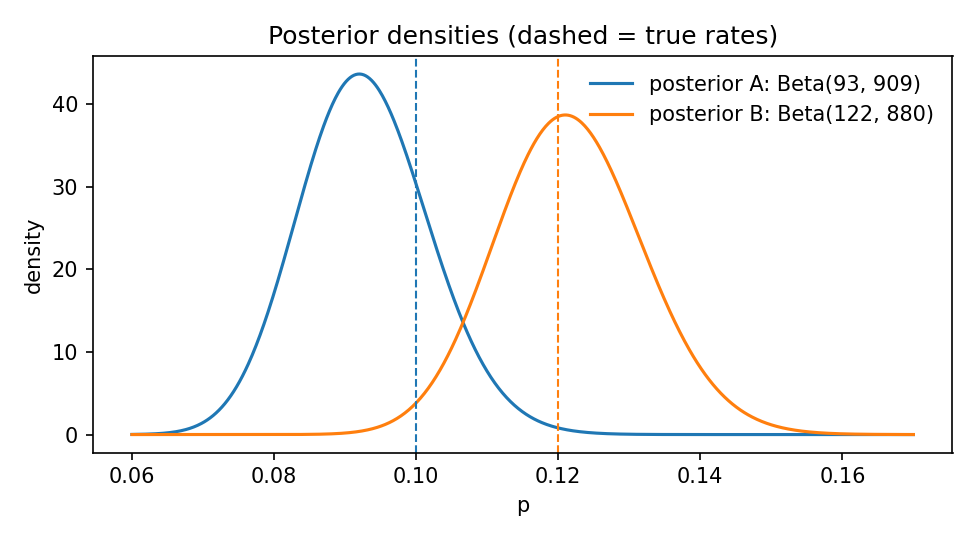
\includegraphics[width=0.62\textwidth]{posteriors.png}
\caption{Posterior densities for the simulated data; the dashed lines are the true rates $0.10$ and $0.12$.}
\end{figure}

\begin{figure}[h]\centering
\begin{minipage}{0.48\textwidth}\centering
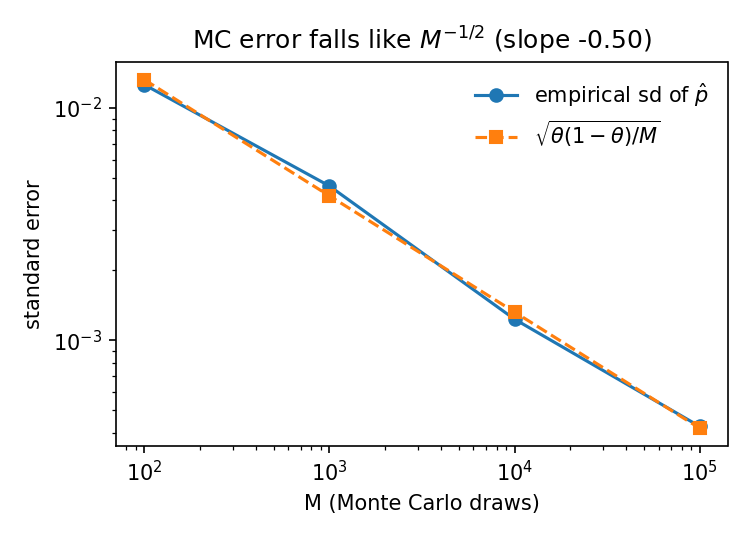
\includegraphics[width=\textwidth]{mc_se.png}
\caption{Empirical SE of $\hat\theta_M$ against $M$ on log--log axes, with the theoretical
$\sqrt{\theta(1-\theta)/M}$.}\label{fig:mcse}
\end{minipage}\hfill
\begin{minipage}{0.48\textwidth}\centering
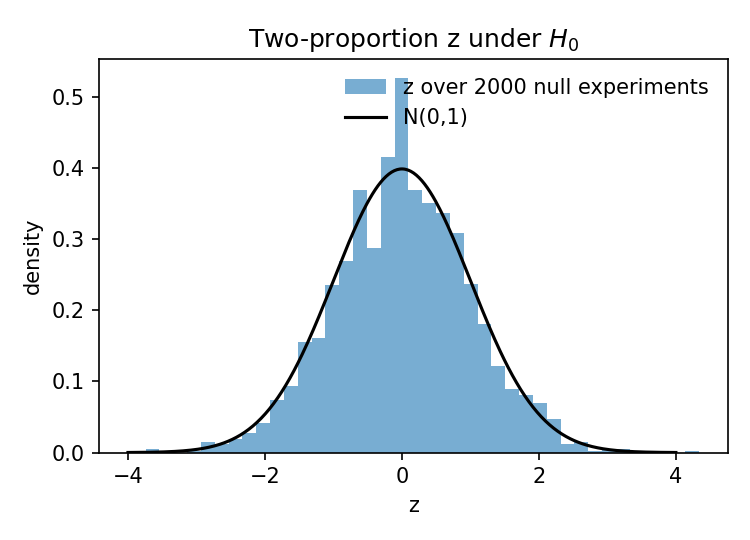
\includegraphics[width=\textwidth]{z_null_hist.png}
\caption{Distribution of $z$ over $2000$ experiments with $p_A=p_B$, against the $N(0,1)$ density.}\label{fig:znull}
\end{minipage}
\end{figure}


\paragraph{Changes in the final implementation.}
\begin{itemize}[nosep]
\item \emph{Posterior draws.} The simulation above drew from the posterior with \texttt{scipy.stats.beta.rvs}. The
  final code is NumPy only, so each draw is $p=G_1/(G_1+G_2)$ with Gamma draws from NumPy and seed~1 for the Monte
  Carlo stream. The Monte Carlo estimate therefore changes from $0.9819$ to $\simThetaMC$; both are within two
  standard errors of the exact value $0.9821$.
\item \emph{Numerical integration.} The simulation above evaluated Proposition~\ref{prop:theta} with SciPy's Beta CDF
  and a trapezoid rule. The final code uses a from-scratch Simpson rule (\texttt{my\_grid\_prob}); SciPy's
  \texttt{quad} is used only to check it.
\item \emph{Null repetitions.} The size of the $z$ test is checked with $1000$ repetitions in \S\ref{sec:it3-sim}
  instead of $2000$.
\end{itemize}

% =====================================================================
\section{Reproducing the results}\label{sec:repro}
\begin{sloppypar}
\noindent Code:\\
\url{https://github.com/amiyasekhar/ds5020-bayesian-ab-testing}\\
The data file (Kaggle, ``Mobile Games A/B Testing -- Cookie Cats'') is not in the repository; save it as
\texttt{data/cookie\_cats.csv}. Requirements: \texttt{numpy}, \texttt{scipy}, \texttt{pandas}, \texttt{matplotlib}.
Run the scripts from the repository root:
\end{sloppypar}
\begin{center}\small
\begin{tabular}{l p{9cm}}\toprule
script & what it produces\\ \midrule
\texttt{src/load\_data.py} & data description: \texttt{docs/data\_macros.tex}, \texttt{data\_summary.tex}, figures\\
\texttt{src/simulation.py} & Appendix~\ref{sec:sim}: \texttt{docs/sim\_macros.tex}, \texttt{sim\_tables.tex}, figures\\
\texttt{src/small\_example.py} & hand-worked example: \texttt{docs/it3\_small.tex}\\
\texttt{src/check\_simulation.py} & simulation test and stress test: \texttt{docs/it3\_sim*.tex}, figures\\
\texttt{src/run\_real.py} & real data and library comparison: \texttt{docs/it3\_real*.tex}, figures\\
\texttt{src/check\_assumptions.py} & assumption checks: \texttt{docs/it3\_assump.tex}\\
\bottomrule\end{tabular}\normalsize
\end{center}
Every number in this report is read from these generated files, so re-running the scripts updates the report.
The simulated data use \texttt{np.random.default\_rng(0)} and the Monte Carlo draws use seed~1.

\end{document}
